\documentclass[12pt]{article}

%\usepackage[utf8]{inputenc}
\usepackage{indentfirst}
\usepackage[hidelinks]{hyperref}
\usepackage{float}
\usepackage{array}
\usepackage{listings}
\usepackage{csquotes}
\usepackage{hyperref}
\usepackage{enumitem, amsmath, amssymb, amsfonts, latexsym, mathrsfs}
\usepackage{graphicx}
\usepackage{subfig}
%\usepackage[greek,english]{babel}
%\usepackage{alphabeta}
\usepackage{multicol}

\newlist{todolist}{itemize}{2}
\setlist[todolist]{label=$\square$}
\usepackage{pifont}
\newcommand{\cmark}{\ding{51}}%
\newcommand{\xmark}{\ding{55}}%
\newcommand{\done}{\rlap{$\square$}{\raisebox{2pt}{\large\hspace{1pt}\cmark}}%
\hspace{-2.5pt}}
\newcommand{\wontfix}{\rlap{$\square$}{\large\hspace{1pt}\xmark}}

\date{}
% Comand para keywords
\providecommand{\keywords}[1]
{
  \small
  \textbf{\textit{Keywords---}} #1
}

% Setup de hiperenlaces
\hypersetup{
    colorlinks=true,
    linkcolor=cyan,
    filecolor=magenta,
    urlcolor=cyan,
    pdftitle={GodOfJustice},
    pdfpagemode=FullScreen,
    }

% Tipografía
\usepackage{helvet}
\renewcommand{\familydefault}{\sfdefault}
\usepackage[sfdefault]{inter}
\usepackage{comment}

% Listas
%\newlist{todolist}{itemize}{2}
%\setlist[todolist]{label=$\square$}

% Imagenes
\graphicspath{ {./images/} }

% Interlineado
\usepackage{setspace}
\spacing{1.5}

% Márgenes
\usepackage[a4paper]{geometry}
\geometry{top=2.5cm, bottom=2.5cm, left=2cm, right=2cm}

% Número de página
\usepackage{fancyhdr}
\pagestyle{fancy}
\rhead[]{}
\lhead[]{}
\renewcommand{\headrulewidth}{0pt}
\rfoot[]{\thepage}
\cfoot[]{}

%_____________________________________________________________________________
%_____________________________________________________________________________
%_____________________________________________________________________________
%_____________________________________________________________________________
\begin{document}

% PORTADA
    \begin{titlepage}

        \centering
        \hrule
        %\vspace{1cm}
        %{\bfseries\Large UNIVERSIDAT JAUME I \par}
        \vspace{1cm}
        {\bfseries\huge Analisis Artistico de the legend of Zelda \par}
        \vspace{3cm}
        {
\includegraphics[width=0.7\textwidth]{images/UJI_logo.jpg} \par}
        \vspace{4cm}
        %{\LARGE \textbf{Deadlyrup} \par}

        {\large
        Nerea Villarrolla Marco \\
        Saul Pacheco Trilles \\
        Alonso Madrigal Hernández \\
        Carlos Castell Campos \\
        Jesus Jimenez Montero \\
        Raul Montero Piñeiro \\
        Selena Monforte Arques \\
        Joan Ruiz Berengue \\
        \par}
        \vspace{10cm}
        \hrule

    \end{titlepage}

 % abstract
\newpage
\begin{abstract}
    En el siguiente documento hablaremos sobre las bases artisticas del videojuego "The Legend Of Zelda: Breath of the wild". Tanto del director de concept art como un atisbo de información sobre el juego. Finalemnete acabaremos con el analisis artistico profundo de varios fan arts.

\end{abstract}

\keywords{Videojuego, arte, concept art, analisis}

% ÍNDICE
%\renewcommand{\tableofcontents}{Indice general}
\newpage
\tableofcontents
\setcounter{tocdepth}{4}

\newpage
%-----------------------------------------------------------------
%-----------------------------------------------------------------
% Tabla de figuras
\newpage
\renewcommand{\listfigurename}{Lita de figuras}
\thispagestyle{empty}
\listoffigures

%-----------------------------------------------------------------
%-----------------------------------------------------------------

\newpage
\section{Introducción}
    \hrule
\vspace{1cm}
    En el siguiente documento queda expuesto nuestro trabajo a lo largo de la asignatura: VJ1204. El cual ha sido un analisis profundo de las diferentes caracteristicas y aspectos que conlleva realizar una composición. Tendremos en cuenta todos estos puntos:
    \begin{itemize}
        \item Perpectiva; línea de horzionte, tupo de vista y puntos de fuga.
        \item Composición; regla de los 2/3, puntos de interes, recorridos visuales, ley de la balanza y simetria.
        \item Claroscuro; clave de la imagen, zonas de iluminación, profundidad, fuente de luz.
        \item Color; gama de colores, tonalidad general, tipos de contraste y colores empleados en primer y segundo plano.
    \end{itemize}

    En una primera parte daremos una pequeña introducción sobre el juego además de dar mención del director de arte principal, el cual fue el que creo los primeros concepts arts de tanto el juego como los personajes. Despues pasaremos ha hablar sobre algunas relaciones conceptuales de diferentes disciplinas, pues en el juego se pueden ver diferentes tipos de arquitecturas que hacen referencia a algunas de la vida real, metodos de arte en el juego que brinda al mundo de hyrule una personalidad única...
\section{El juego}
    \hrule
\vspace{1cm}
The Legend Of Zelda: Breath of the wild es la décima octava entrega de la saga The Legend of Zelda. Lanzado en el 2017 por Nintendo en la consola Nintendo switch y la WII U, esta entrega nos brinda un mundo abierto lleno de cosas por hacer. Podemos ir directamente por el jefe final, o podemos perdernos por el colosal e interesante mundo. Yendo a los sitios más reconditos e intrincados de llegar.
    El mundo esta embadurnado de secretos, personajes interesantes, misterios por descubrir y batallas que librar. Este titlo ha sido aclamado por la critica desde su salida, siendo para muchos uno de los mejores titulos que hayan podido jugar. Pero sus afirmaciones no son fundamentos sin una base solida y es que Breath of the wild, tiene notas que no bajan del nueve por más de 14 revistas. Ganó 5 premios entre ellos el GOTY y mejor dirección de juego. Y es que este juego ha sido un punto y aparte en los videojuegos, un ejemplo a seguir de como ha de realizarse un mundo abierto.

\subsection{Satoru Takizawa}
Comenzó creando el logo de Yoshi's Island 2, pero acabo creando las bases más importantes de la saga Zelda, y e que Satoru ha creado el diseño del proprio Ganondorf, el villano principal de toda la saga. También ha dado vida a varios enemigos menores de la saga Mario bros que se han vuelto marca insignia de los juegos del fontanero. Para el titulo The Legend of Zelda: Twilight Princess, Satoru fue nombrado director de arte del juego, siendo este su primer trabajo en este rol. Despues debido a su excelente trabajo se siguió nombrando a el para desempeñar este rol, siendo uno de esos trabajos The Legend of Zelda: Breath of the Wild.
\section{Relaciones Conceptuales}
    \hrule
\vspace{1cm}

\subsection{Arquitectura}

\subsection{Arte}

\subsection{Fotografía}

\subsection{La música}
Se tiene en cuenta que la mayoría de las travesías en la aventura, nos invade el silencio o los sonidos ambientales de los pájaros o más animales. Pero la música de ZBoW juega un gran papel en lo que es el game feel. Ya que en este juego a pesar de momentos puntuales no hace uso de grandes orquestas filarmónicas, si no de serenas melodías que nos ayudan a situarnos tanto geográficamente como temporalmente. Suaves flautas y oboes en la ciudad gerudo con el toque desértico que nos evocan a montañas de arena. Música con fuerte repercusión en la ciudad Goron, pero ninguna de estas opacando la acción del protagonista, si no más bien acompañándolo serenamente.

%-----------------------------------------------------------------
%-----------------------------------------------------------------


\section{Analisis conceptual de imágenes}
    \hrule
\vspace{1cm}
    \subsection{1. Nerea}
        \subsubsection{Perspectiva}

        \subsubsection{Composición}

        \subsubsection{Clarooscuro}

        \subsubsection{Color}
        \newpage

%-----------------------------------------------------------------
%-----------------------------------------------------------------

    \subsection{2. Jesús}
        \subsubsection{Perspectiva}

        \subsubsection{Composición}

        \subsubsection{Clarooscuro}

        \subsubsection{Color}
        \newpage

%-----------------------------------------------------------------
%-----------------------------------------------------------------

    \subsection{3. Saul}
    \begin{figure}[H]
      \centering
      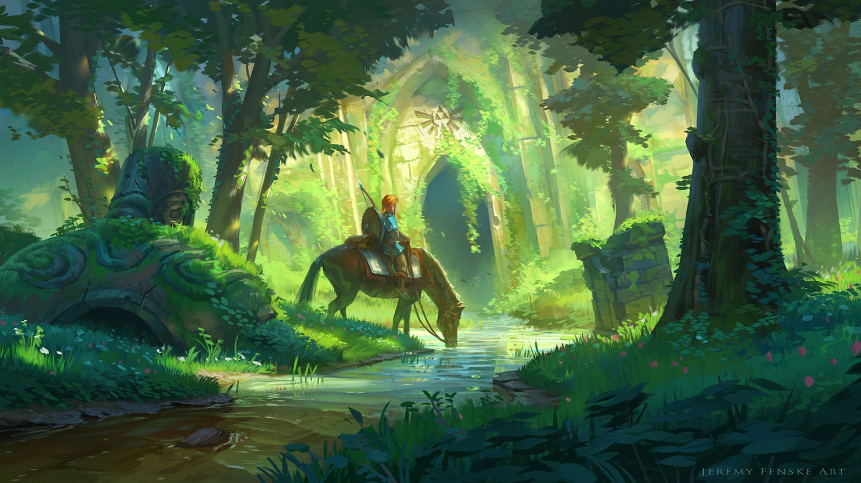
\includegraphics[scale=0.7]{images/Saúl/Sección 3/EA_img3_0Main.png}
      \caption{\small 4.3.3. Imagen}
    \end{figure}
    Se trata de una imagen oficial del juego, y se compone por el personaje principal montado a su caballo Epona.

    
        \subsubsection{Análisis de la perspectiva}


    \begin{figure}[H]
      \centering
      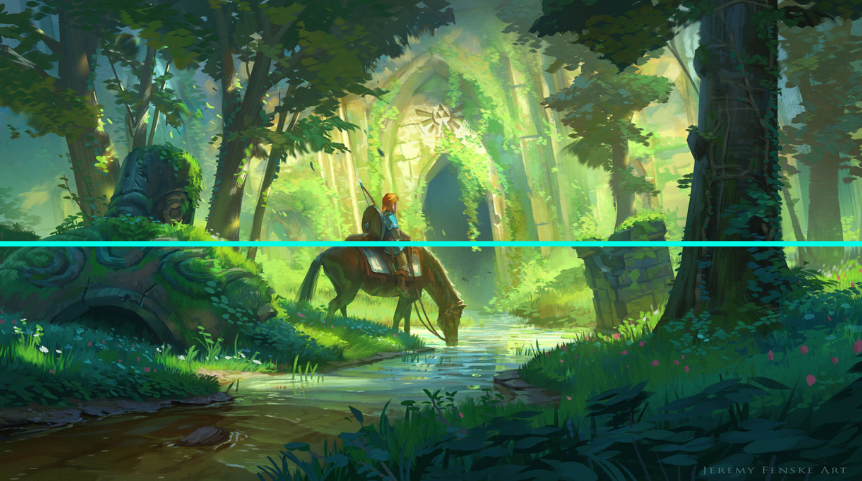
\includegraphics[scale=0.7]{images/Saúl/Sección 3/EA_img3_1Perspectiva_1LineaTierra-TipoVista.png}
      \caption{\small 4.3.1.1 Línea del horizonte y tipo de vista}
    \end{figure}

    La línea del horizonte se halla sobre una altura media e incluso si afinamos mucho se puede apreciar que está ligeramente desplazada hacia arriba. Como la línea del horizonte se encuentra en la zona central de la ilustración podemos afirmar que estamos ante una vista serena.

    \begin{figure}[H]
      \centering
      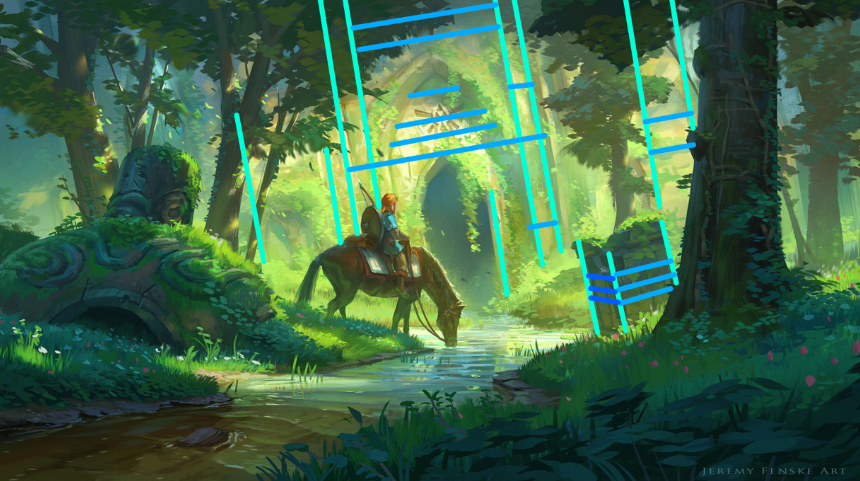
\includegraphics[scale=0.7]{images/Saúl/Sección 3/EA_img3_1Perspectiva_2PuntosFuga.png}
      \caption{\small 4.3.1.2 Puntos de fuga}
    \end{figure}

    Aunque en la mayoría de la imagen predomina la naturaleza al fondo se puede apreciar un antiguo edificio en el cual podemos encontrar hasta dos puntos de fuga ya que solo vemos una fachada y está algo inclinada. Además si nos fijamos bien, más adelante encontramos una ruina de una columna en la que sí se puede llegar a apreciar los tres puntos de fuga. Sin embargo en el resto de la imagen no se pueden apreciar más puntos de fuga ya que como he dicho antes predomina la naturaleza.
(Estos puntos de fuga están todos fuera de la ilustración por lo que se han marcado con distintos colores las líneas que irían al punto de fuga pero no se han alargado en todos los casos para no entorpecer a la vista).


        \subsubsection{Análisis de la composición}

        
    \begin{figure}[H]
      \centering
      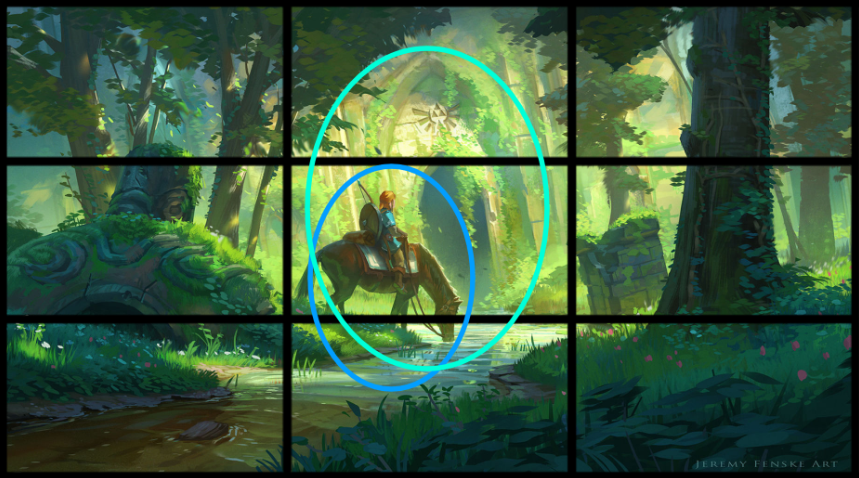
\includegraphics[scale=0.7]{images/Saúl/Sección 3/EA_img3_2Composicion_1Regla2-3.png}
      \caption{\small 4.3.2.1 Regla de los 2/3}
    \end{figure}

En esta ilustración podemos apreciar como los elementos principales se encuentran en el centro de la imagen. Además como podemos ver el personaje principal está contenido en la sección del centro de esta regla de los 2/3.

    \begin{figure}[H]
      \centering
      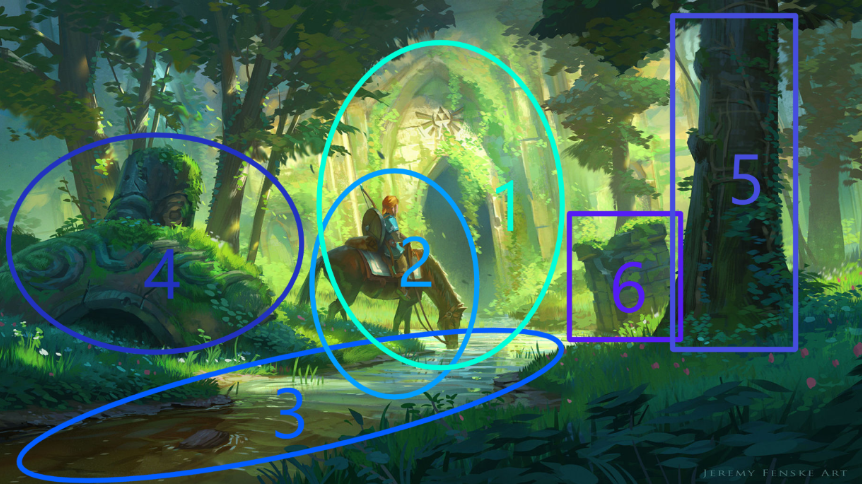
\includegraphics[scale=0.7]{images/Saúl/Sección 3/EA_img3_2Composicion_2PuntosInteres.png}
      \caption{\small 4.3.2.2 Centro de interés, principal y secundarios}
    \end{figure}

Los principales puntos de interés son en primer lugar el templo al que le está lloviendo toda la luz de la imagen indicando que este es uno de los elementos más importantes y en segundo lugar es Link el personaje principal con el caballo quedándose con algo de esa luz que recibe el primer punto de interés, luego ya como puntos de interés secundarios tenemos en tercer lugar el río marcando un poco la ruta visual tema que trataremos ahora en la siguiente diapositiva, luego ya tenemos en el cuarto círculo un guardián y luego ya el quinto punto con el árbol ocupando la parte de la derecha de la ilustración y por último casi sin importancia las ruinas de la columna que corresponde al sexto punto de interés

    \begin{figure}[H]
      \centering
      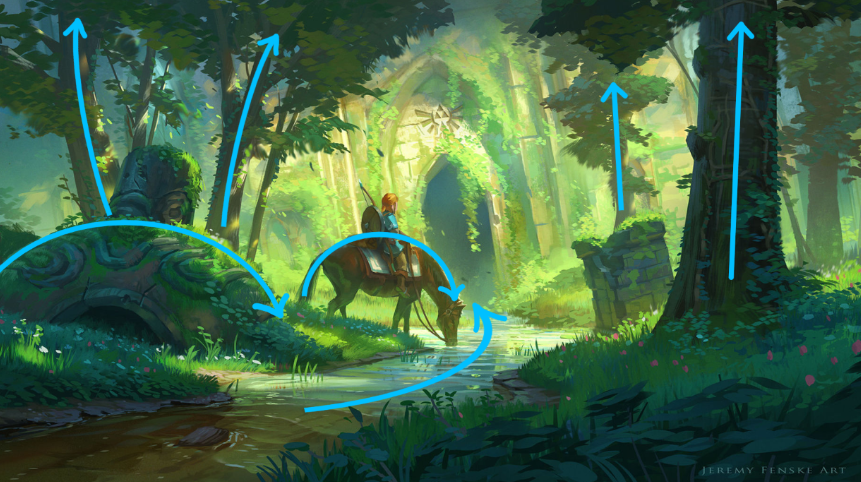
\includegraphics[scale=0.7]{images/Saúl/Sección 3/EA_img3_2Composicion_3RutaVisual.png}
      \caption{\small 4.3.2.3 Ruta visual}
    \end{figure}

 En esta ilustración podemos apreciar como la principal ruta visual es el río que va desde abajo a la izquierda recorriendo toda la imagen hasta dentro del templo con la ayuda del personaje principal que trae la atención de la parte izquierda de la imagen, luego por otro lado están los árboles que son elementos importantes para el recorrido visual estos tiran la vista hacia el cielo intuyo que para dirigirte la mirada a donde hay luz y la luz te vuelva a dirigir dentro del templo ya que el templo está iluminado con toda esta luz haciendo que gane mucha relevancia.

    \begin{figure}[H]
      \centering
      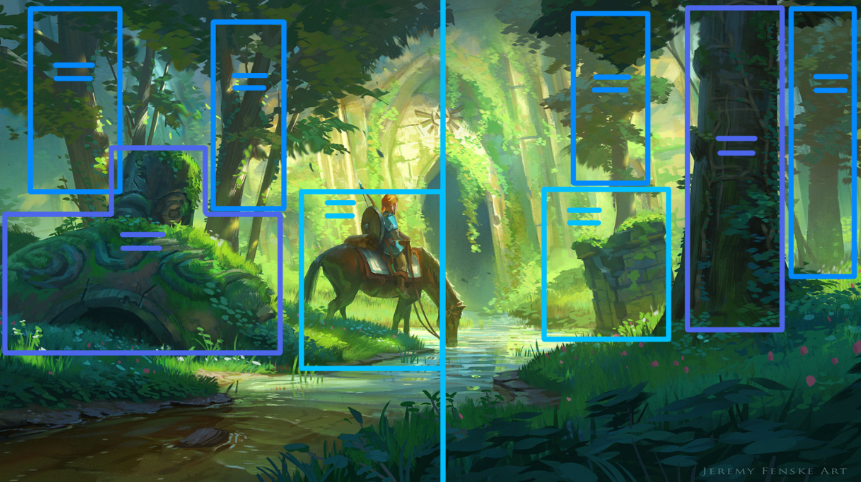
\includegraphics[scale=0.7]{images/Saúl/Sección 3/EA_img3_2Composicion_4LeyBalanza-Simetria.png}
      \caption{\small 4.3.2.4 Ley de la balanza, equilibrio de pesos y simetría vs asimetría}
    \end{figure}

Esta ilustración cumple con la ley de la balanza ya que si partimos la imagen por la mitad más o menos los elementos que componen la imagen tienen el mismo peso, marcados con colores nos podemos fijar que están el personaje con el caballo y al otro lado la ruina de la columna en el azul-morado tenemos a el árbol grande y haciéndole el contrapeso el guardián y por último tenemos a los 4 árboles del fondo que estos además de tener el mismo peso son simétricos. De hecho la imagen en sí guarda bastante simétrica solo hay que mirar la disposición de los colores están azul oscuro morado azul oscuro y azul claro y en el otro lado del eje de simetría están igual.



        \subsubsection{Claroscuro}

        
    \begin{figure}[H]
      \centering
      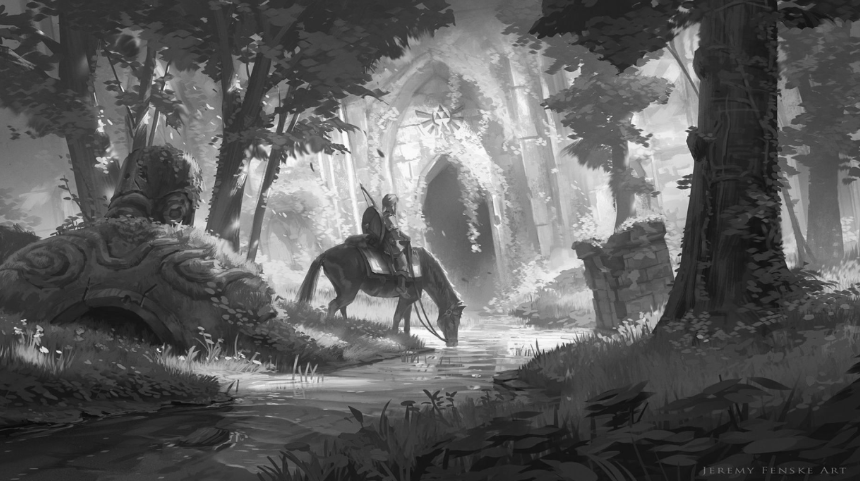
\includegraphics[scale=0.7]{images/Saúl/Sección 3/EA_img3_3Claroscuro_1Profundidad.png}
      \caption{\small 4.3.3.1 Uso del claroscuro para representar la profundidad}
    \end{figure}

A nivel del claroscuro, podemos apreciar que la zona más oscuras se sitúan en el primer plano y luego la zona de profundidad donde tenemos una clave alta es decir con más luminosidad esta se sitúa en la parte más lejana, lo que produce un contraste y crea esa sensación de profundidad en la imagen.

    \begin{figure}[H]
      \centering
      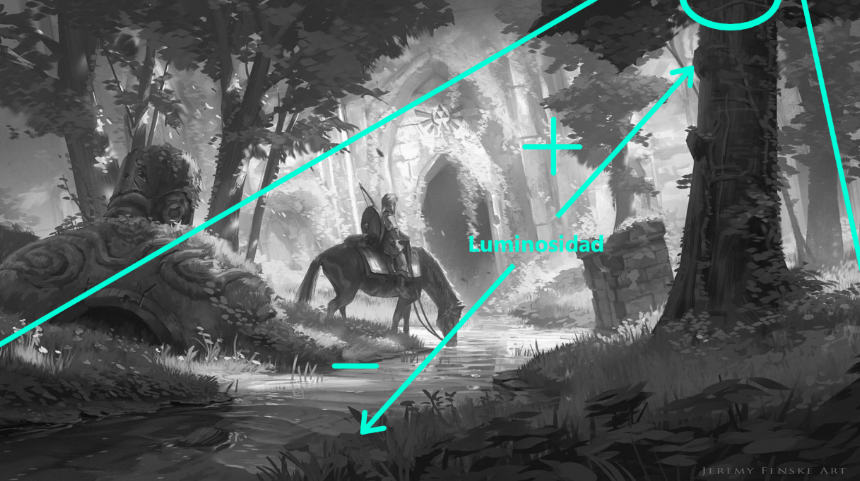
\includegraphics[scale=0.7]{images/Saúl/Sección 3/EA_img3_3Claroscuro_2Luminosidad.png}
      \caption{\small 4.3.3.2 Zonas más luminosas y menos, y ubicación de la fuente de iluminación}
    \end{figure}

En esta imagen tenemos dos zonas, la zona de clave alta que sería la que está más al fondo con mucha luz y luminosidad y luego la zona de clave baja que se sitúa en el primer plano y la que está bañada con todas esas sombras. La ubicación de la fuente de luz, es la semicircunferencia que tenemos arriba a la derecha en dirección a la mayor luminosidad.

    \begin{figure}[H]
      \centering
      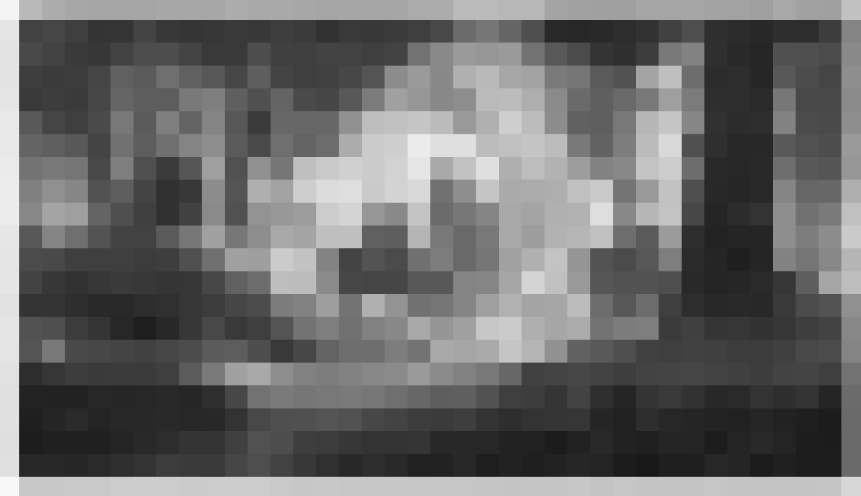
\includegraphics[scale=0.7]{images/Saúl/Sección 3/EA_img3_3Claroscuro_3Clave.png}
      \caption{\small 4.3.3.3 Clave de la imagen}
    \end{figure}

Esta ilustración es una clave media, ya que aunque existen dos zonas bien diferenciadas como son el primer plano con una clave baja y la zona de profundidad con una clave alta, Al pixelar la imagen con los niveles de grises, podemos apreciar con mayor claridad que no hay ninguno que predomine sobre el otro hay más o menos la misma cantidad de claro que de oscuro, es por ello que la ilustración es una clave media.

        \subsubsection{Color}


    \begin{figure}[H]
      \centering
      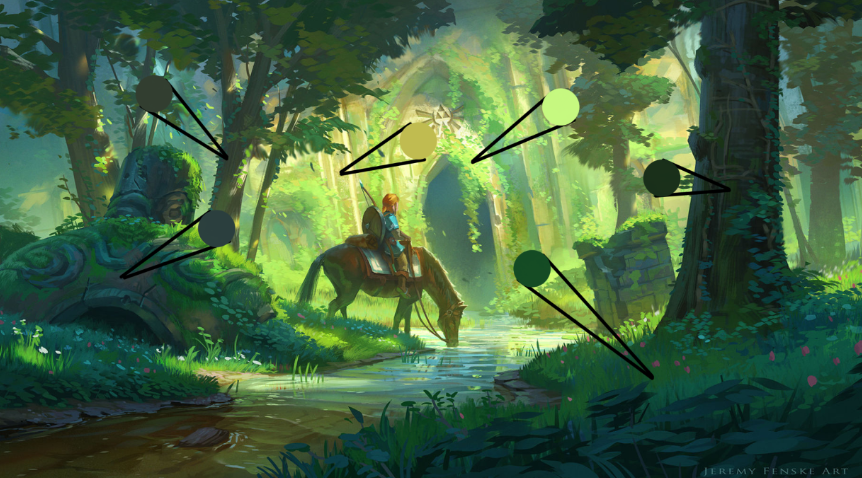
\includegraphics[scale=0.7]{images/Saúl/Sección 3/EA_img3_4Color_1TonalidadGenral.png}
      \caption{\small 4.3.4.1 Tonalidad de color global}
    \end{figure}

La imagen tiene una tonalidad de color global fría pero no es su totalidad ya que esta compuesta por las diferentes tonalidades de verdes (que seria la parte fria que envuelve toda la imagen) y los diferentes tonos de amarillos que destacan dada la excesiva luminosidad que reciben (esta seria la parte calida de la imagen). Hay un gran balance entre ambos colores pero sin embargo predomina al ojo el verde porque es el color que mejor percibimos, por eso tiene una tonalidad fría.

    \begin{figure}[H]
      \centering
      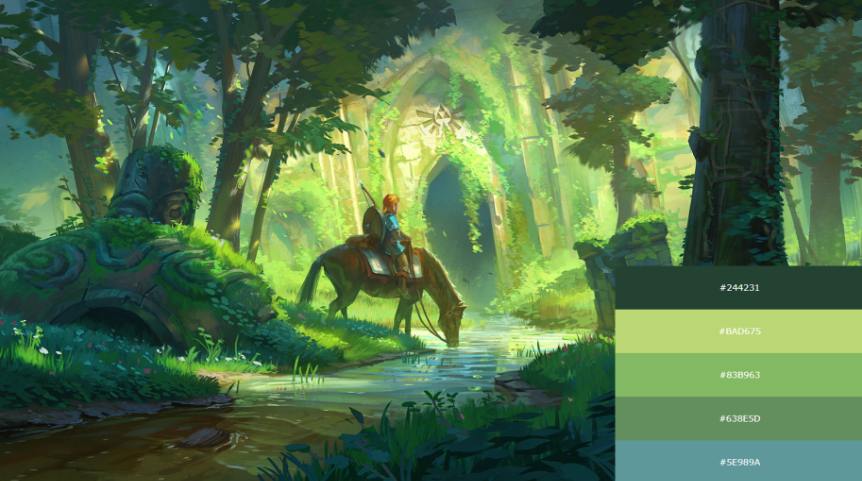
\includegraphics[scale=0.7]{images/Saúl/Sección 3/EA_img3_4Color_2GamaColores.png}
      \caption{\small 4.3.4.2 Gama de color empleada}
    \end{figure}

La gama de colores empleada en esta imagen consta de una gama de tonalidades de verdes analogos entre ellos, incluso llegando a ampliar hasta algun amarillo en la fachada de las ruinas del templo del fondo. Sin embargo el cambio entre estos dos colores es muy suave puesto que el verde es un color secundario procedente del amarillo.

    \begin{figure}[H]
      \centering
      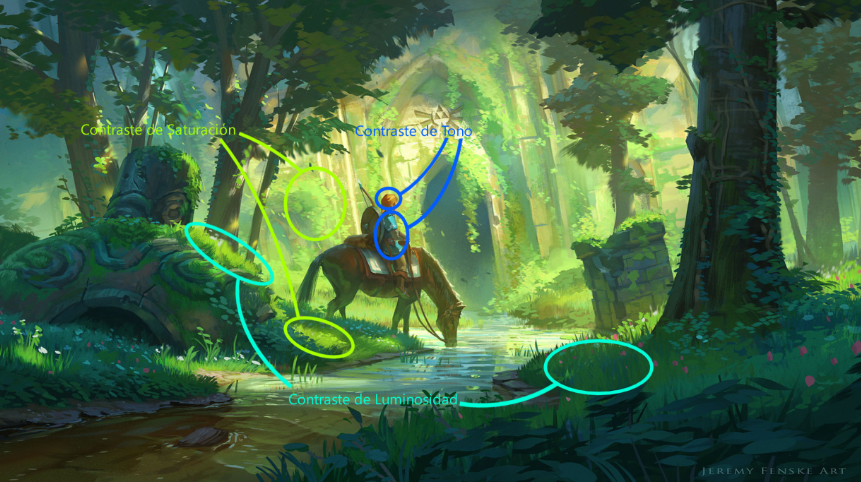
\includegraphics[scale=0.7]{images/Saúl/Sección 3/EA_img3_4Color_3Contrastes.png}
      \caption{\small 4.3.4.3 Tipos de contraste}
    \end{figure}

En el contraste de saturación podemos encontrar una diferencia de intensidad del color entre dos o más elementos visuales en este caso en la imagen he marcado dos verdes uno más próximo a los primeros planos y el otro en el plano del fondo. El contraste de tono es la diferencia en el tono o matiz del color entre dos o más elementos visuales, esto se da entre colores cálidos y colores fríos, por ellos he marcado los colores complementarios del pelo del protagonista y la ropa del mismo. El contraste de luminosidad es la diferencia en el brillo o la luminosidad entre dos o más elementos visuales. Este se utiliza para destacar ciertos elementos o para crear una sensación de profundidad, por ello he marcado dos tonalidades de verde que están en distintos planos de profundidad uno al fondo y otro en el primer plano.

    \begin{figure}[H]
      \centering
      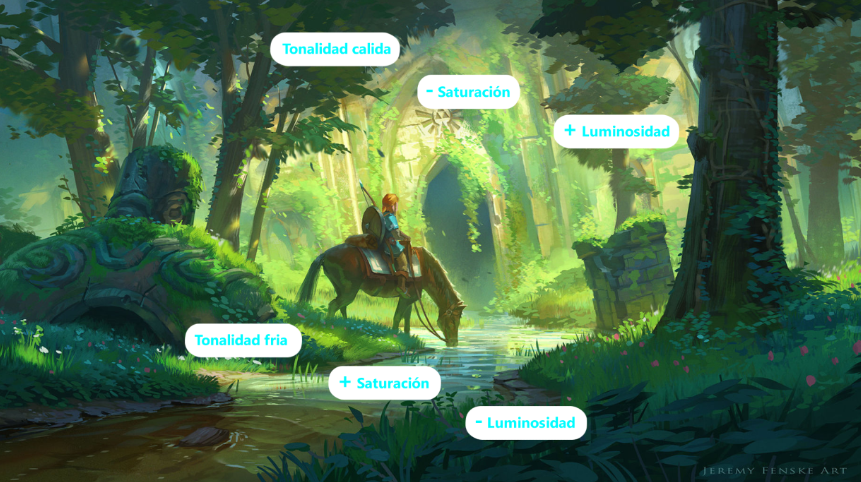
\includegraphics[scale=0.7]{images/Saúl/Sección 3/EA_img3_4Color_4AnalisisPlanosPrimeroFondo.png}
      \caption{\small 4.3.4.4 Análisis de los colores empleados en primer y último plano}
    \end{figure}

En esta ilustración podemos ver como los colores utilizados en el primer plano estan bastante mas saturados que los se encuentran al fondo de la ilustración y pasa al contrario con la luminosidad que en el primer plano nos encontramos con colores con menos luminosidad y al fondo con más luminosidad. Por tanto esto nos deja con unos colores más claros y menos saturados en el último plano para crear una sensación de profundidad y hacer que los elementos del primer plano se destaquen o llamen la atención. Por otro lado pasa lo mismo con la tonalidad, se utilizan tonos fríos en el primer plano y tonos cálidos en el último plano para crear esa sensación de profundidad.
        \newpage

%-----------------------------------------------------------------
%-----------------------------------------------------------------

    \subsection{4. Raúl}
        \subsubsection{Perspectiva}

        \subsubsection{Composición}

        \subsubsection{Clarooscuro}

        \subsubsection{Color}
        \newpage

%-----------------------------------------------------------------
%-----------------------------------------------------------------

    \subsection{5. Miquel}
        \subsubsection{Perspectiva}

        \subsubsection{Composición}

        \subsubsection{Clarooscuro}

        \subsubsection{Color}
        \newpage

%-----------------------------------------------------------------
%-----------------------------------------------------------------

    \subsection{6. Nerea (segunda imagen)}
        \subsubsection{Perspectiva}

        \subsubsection{Composición}

        \subsubsection{Clarooscuro}

        \subsubsection{Color}
        \newpage

%-----------------------------------------------------------------
%-----------------------------------------------------------------

    \subsection{7. Miquel (segunda imagen)}
        \subsubsection{Perspectiva}

        \subsubsection{Composición}

        \subsubsection{Clarooscuro}

        \subsubsection{Color}
        \newpage
%-----------------------------------------------------------------
%-----------------------------------------------------------------

    \subsection{8. Raúl (Segunda imagen)}
        \subsubsection{Perspectiva}

        \subsubsection{Composición}

        \subsubsection{Clarooscuro}

        \subsubsection{Color}
        \newpage

%-----------------------------------------------------------------
%-----------------------------------------------------------------

    \subsection{9. Alonso}
    \begin{figure}[H]
      \centering
      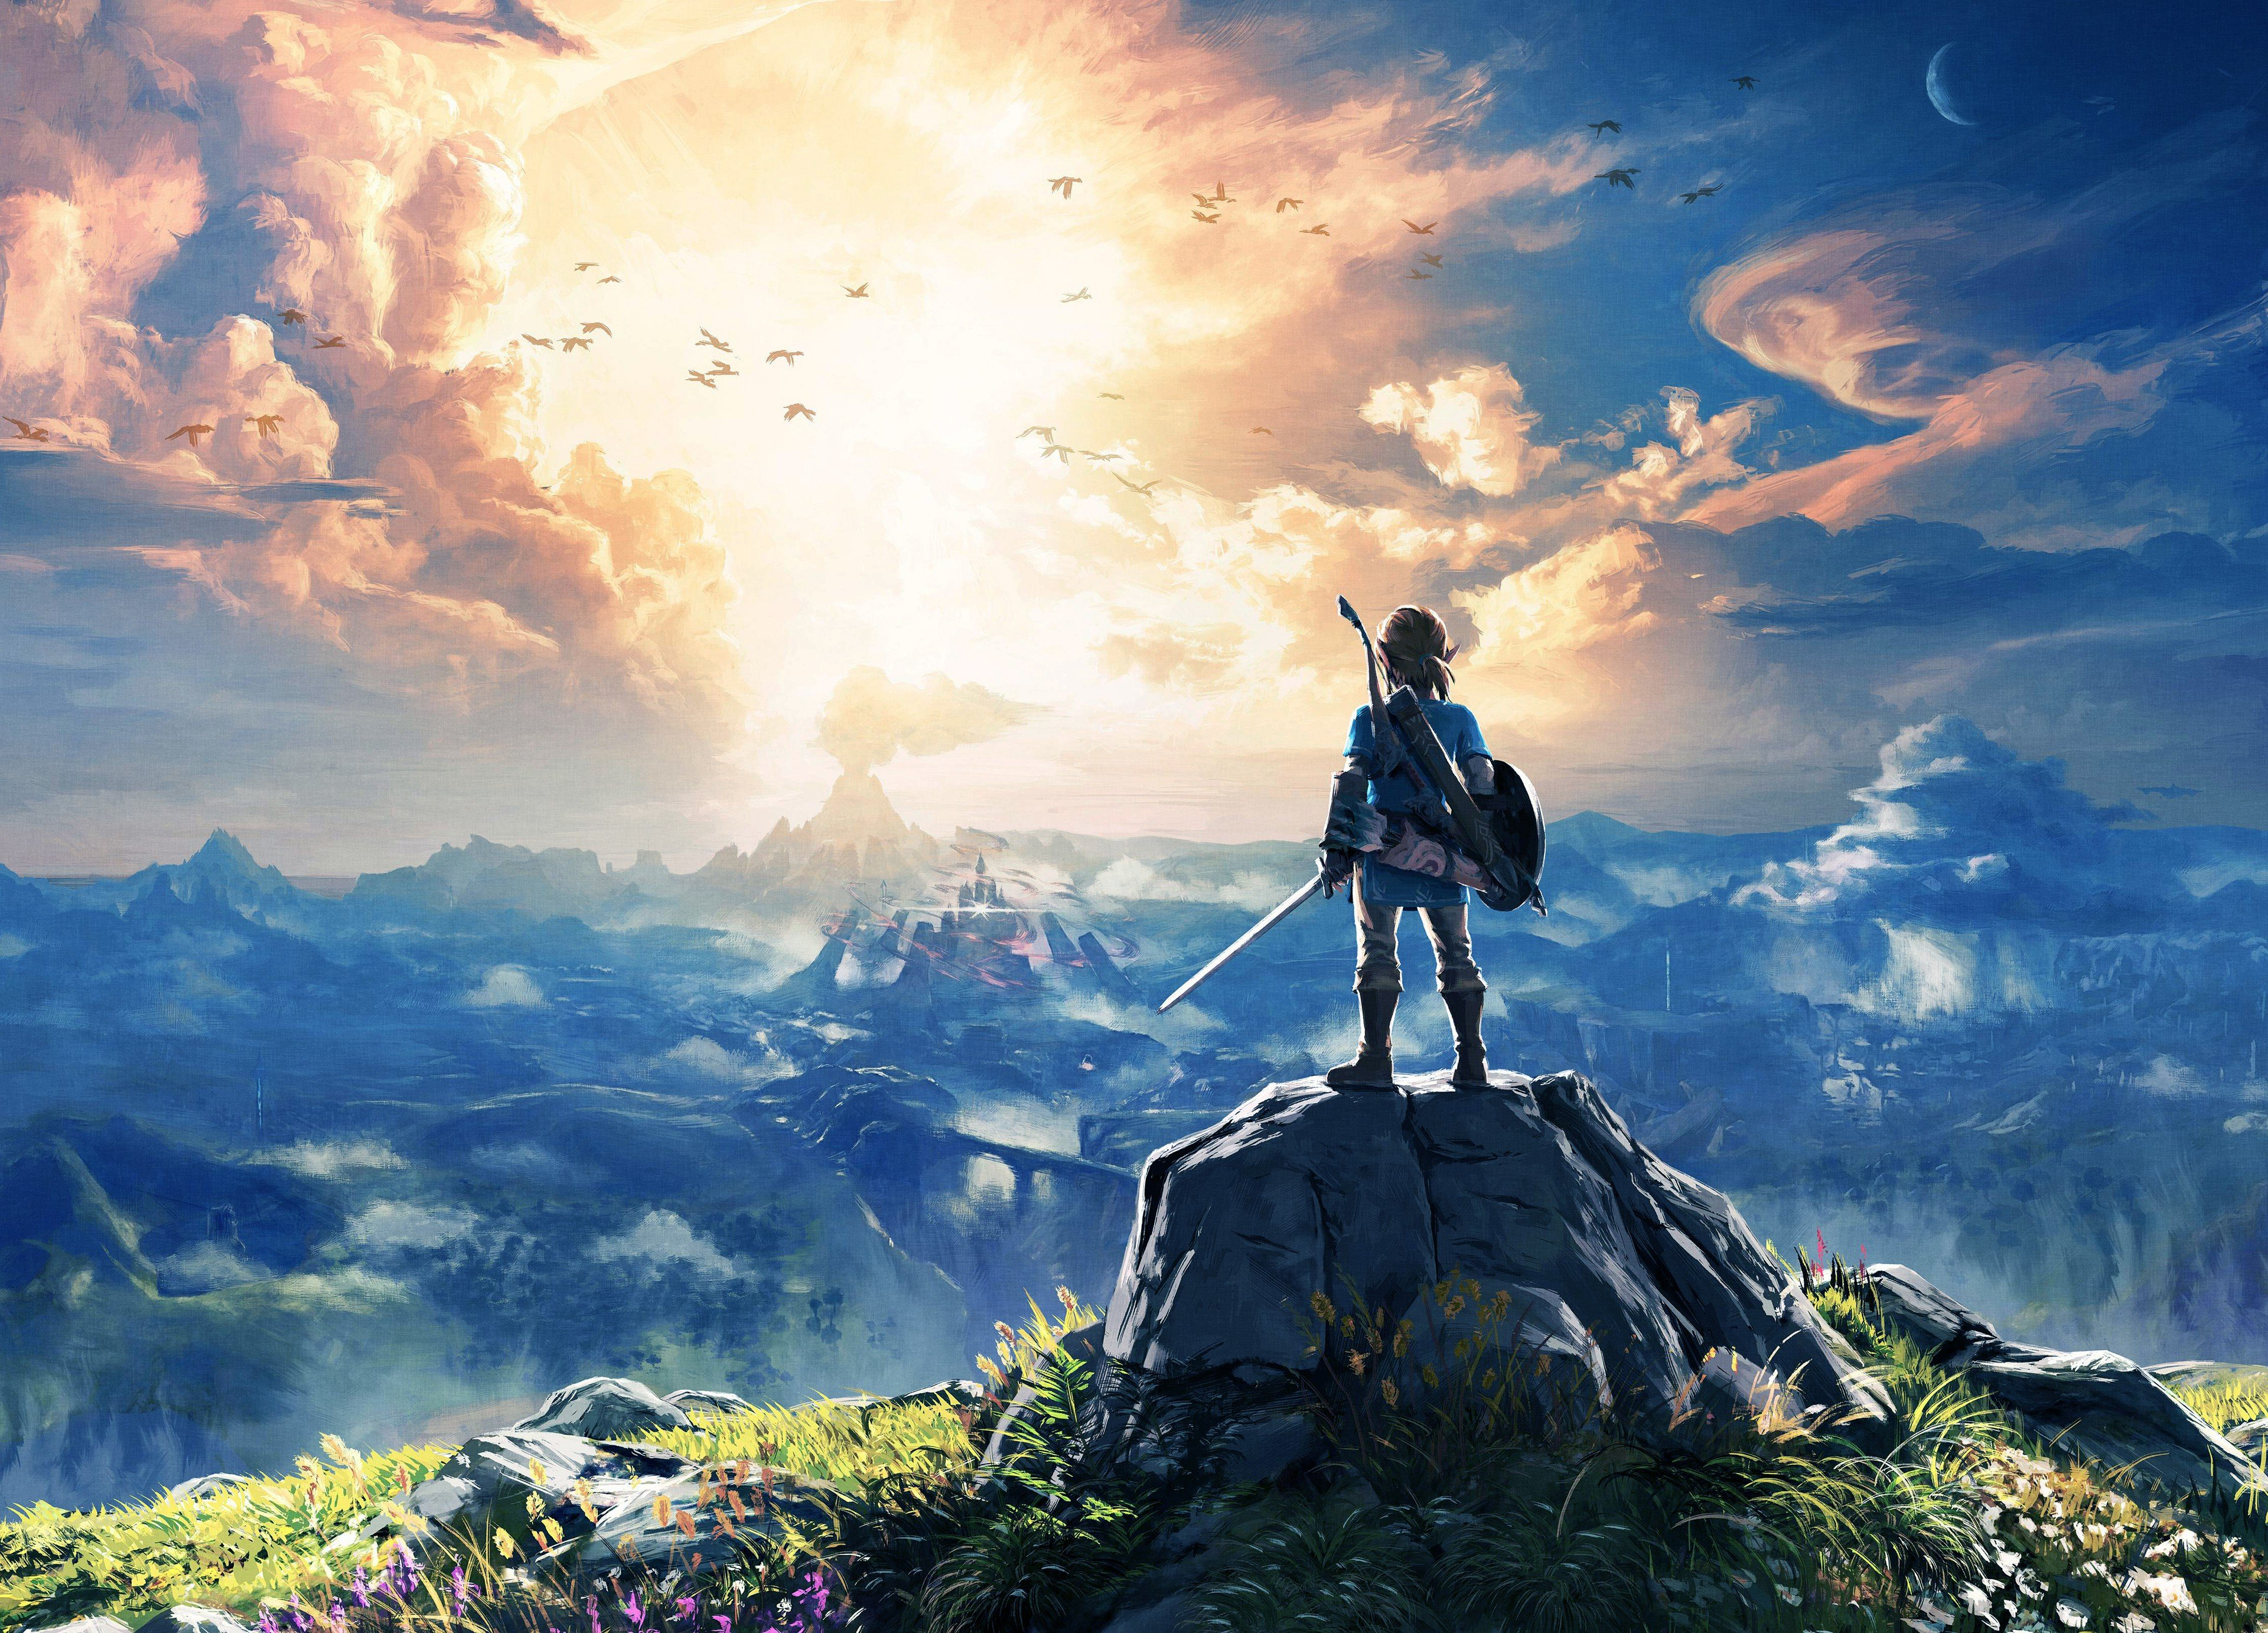
\includegraphics[scale=0.1]{images/Concepts/9_concept_art}
      \caption{\small 9. Imagen}
    \end{figure}
    Se trata de una imagen oficial del juego, la portada del mismo.

        \subsubsection{Perspectiva}

    \begin{figure}[H]
      \centering
      \includegraphics[scale=0.1]{images/Alonso/Sección 9/Linea orizonte}
      \caption{\small 9. Linea del horizonte}
    \end{figure}

    Comenzaremos hablando de la línea del horizonte la cual está situada justo en medio de la imagen. Se puede discernir perfectamente debido a que se encuentra directamente el propio horizonte en la lejanía delimitado por una línea perfectamente recta. En función de estos datos podemos concluir  que se trata de una vista serena.

    \begin{figure}[H]
      \centering
      \includegraphics[scale=0.1]{images/Alonso/Sección 9/caja.jpg}
      \caption{\small 9. puntos de fuga}
    \end{figure}

    Cómo está estructurada la imagen no podremos sacar información de la misma. Los elementos son demasiado orgánicos como para establecer la existencia de puntos de fuga que nos aclaren la perspectiva. Sin embargo si cerramos la piedra en la que se encuentra link en una caja. Sacamos más información pues así dibujado podríamos decir que hay más de un punto de fuga. Aun así la representación de la caja puede llegar a ser demasiado subjetiva. Es por ello que no se puede establecer con exactitud el número de puntos de fuga ni su ubicación.

        \subsubsection{Composición}
    \begin{figure}[H]
      \centering
      \includegraphics[scale=0.1]{images/Alonso/Sección 9/2-3.jpg}
      \caption{\small 9. 2/3}
    \end{figure}
    Con la regla de los 2/3 podremos ver los puntos más notorios de la imagen, pues son aquellos que caen exactamente en las esquinas de los cuadrados que representa esta regla. Señalando y dando protagonismo a 2 puntos de interés. Que prácticamente serían los dos únicos más importantes en toda la imagen.

    \begin{figure}[H]
      \centering
      \includegraphics[scale=0.1]{images/Alonso/Sección 9/Puntos de interes.jpg}
      \caption{\small 9. puntos de interes}
    \end{figure}

    Los puntos de interés, gracias a la regla de los 2/3 podremos señalar tanto el sol que está iluminando a todo Hyrule, es decir, a todos los elementos de la imagen, siendo el propio sol el elemento más iluminado. Y al propio link que se encuentra en la segunda mitad de toda la composición y en un primer plano dándole protagonismo a sí mismo.
    Y son pues estos elementos los primeros a los que acude la mirada en toda la representación. También podríamos marcar como puntos de interés secundarios el castillo de hyrule, el volcán y los pájaros en la parte superior de la imagen. El castillo por tener un destello que marca claramente un punto de interés. Y el volcán señalando con su estructura natural el sol que ilumina toda la escena, acompañado de los pájaros que realizan la misma función.

    \begin{figure}[H]
      \centering
      \includegraphics[scale=0.1]{images/Alonso/Sección 9/recorrido visual.jpg}
      \caption{\small 9. recorrido visual}
    \end{figure}

    Es por ello que el recorrido visual es más claro, Pues los pájaros, el volcán, la propia estructura del castillo de hyrule, la mirada de link y su posición, prácticamente todos los elementos de la composición. Nos dan a entender que el elemento principal es el destello del sol. Mires el elemento que mires te da a entender que hay un elemento más importante y es por ello que te lo está señalando con su propia estructura.

    \begin{figure}[H]
      \centering
      \includegraphics[scale=0.1]{images/Alonso/Sección 9/ley de la balanza.jpg}
      \caption{\small 9. Balanza y simetría}
    \end{figure}

    La ley de la balanza se cumple de forma espléndida, porque ninguno de los elementos principales de la imagen opacan al otro en protagonismo, si no que se podrían considerar igual de notorios e importantes. Pues la luminosidad del potente sol está compensada con la imponente puesta en escena de Link, posando con su espada mirando al horizonte, apoyado con la altura de la roca. Manteniendo los dos elementos la misma cantidad de peso. Con ello se puede aprovechar para decir que no existe ninguna simetría en la imagen, por lo que es asimétrica.

        \subsubsection{Clarooscuro}

    \begin{figure}[H]
      \centering
      \includegraphics[scale=0.1]{images/Alonso/Sección 9/blanco y negro.jpg}
      \caption{\small 9. Blanco y negro}
    \end{figure}
    Con la imagen en blanco y negro podemos hacer un rapido analisis con sus profundidades, se ven claramente 2 profundidades demarcadas de forma muy notoria con la luminosidad, pues las partes en primer plano tienen una clave más baja que la que estan en segundo plano, que adquieren más protagonismo por estar tan iluminadas.

    \begin{figure}[H]
      \centering
      \includegraphics[scale=0.1]{images/Alonso/Sección 9/pixel.jpg}
      \caption{\small 9. Pixel}
    \end{figure}

    Sin embargo cuando pixelamos la imagen nos podemos dar más cuenta de que debido al contraste de luminosidad entre el primer y segundo plano hace una mezcla de valores de color que hace detonar la imagen con una clave media. Pues ninguno de los dos valores de luminosidad resalta sobre el otro.

    \begin{figure}[H]
      \centering
      \includegraphics[scale=0.1]{images/Alonso/Sección 9/luminosidad.jpg}
      \caption{\small 9. Fuente de luz}
    \end{figure}

    Es por el elemento principal de la imagen la causa de la fuente de luminosidad, pues debido a su condición de ser un sol está iluminando a toda la imagen, dejando solo oscura las sombras que provoca esta misma iluminación. Marcadas perfectamente en la imagen.

        \subsubsection{Color}
        \begin{figure}[H]
      \centering
      \includegraphics[scale=0.1]{images/Alonso/Sección 9/Paleta color.jpg}
      \caption{\small 9. paleta de color}
    \end{figure}

        La gama cromática empleada ha resultado finalmente tener una estructura bastante lógica, pues se trata de una triada de colores, debido al verde de la hierba, el azul del cielo y del reino de hyrule y el sol anaranjado. Dan como resultado una triada de colores bastante definidos.
\begin{figure}[H]
      \centering
      \includegraphics[scale=0.1]{images/Alonso/Sección 9/colores.jpg}
      \caption{\small 9. Tonalidad general}
    \end{figure}
    La tonalidad global de la imagen es difícil de determinar, debido a que gracias a su iluminación tan potente, hace un macro contraste de tono entre una tonalidad fría y una tonalidad algo más cálida. Lo que sí podemos describir es la saturación general de los colores presentes en la imagen. Pues el tono es muy intenso dejando una saturación  bastante alta en prácticamente toda la imagen.

\begin{figure}[H]
      \centering
      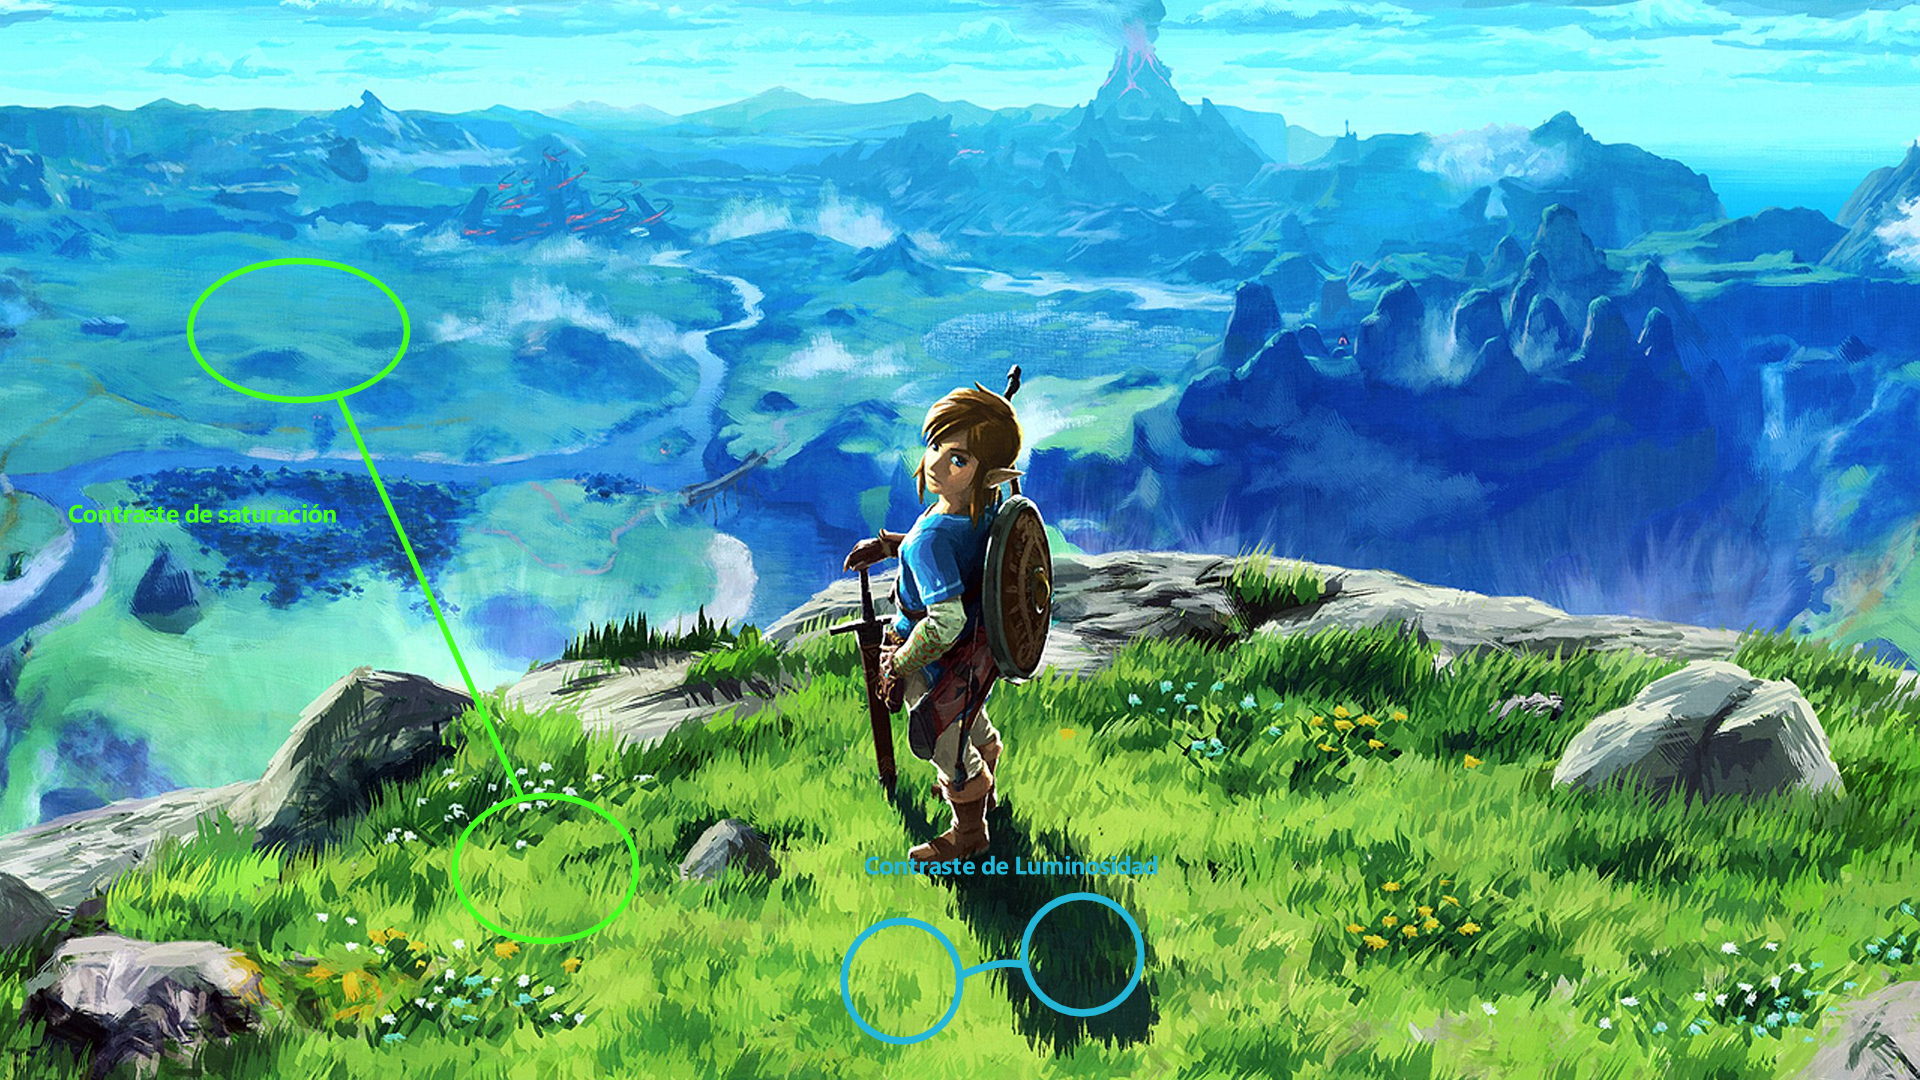
\includegraphics[scale=0.1]{images/Alonso/Sección 9/Contrastes.jpg}
      \caption{\small 9. tipos de contrastes}
    \end{figure}
    Los tipos de contraste en esta imagen son bastante claros en cada uno de sus apartados. Empezando con el Tono, hay un intenso contraste de tonos a lo largo de la representación. Principalmente se trata del contraste entre la luz anaranjada del sol y el azul intenso del cielo. Gracias a la sombra de la piedra provocada por el sol, podemos ver el contraste de luminosidad entre la sombra y la parte iluminada por el foco de luz. Y finalmente hay un ligero contraste de Saturación, pues a medida que nos acercamos al horizonte podemos ver un color mucho más apagado que el del centro del foco.

    \begin{figure}[H]
      \centering
      \includegraphics[scale=0.1]{images/Alonso/Sección 9/analisis de meirda.jpg}
      \caption{\small 9. Analisis de capas}
    \end{figure}

    Por todo lo comentado podemos concluir lo siguiente: Entre el primer y segundo plano hay un contraste de luminosidad y contrastes bastante evidente. El primer plano tiene una luminosidad apagada con una saturación alta, pero poco notable debido a su poca luminosidad. Y en suegundo plano si que podemos ver colores vivos e iluminados, pero con la misma cantidad de saturación.


        \newpage

%-----------------------------------------------------------------
%-----------------------------------------------------------------

    \subsection{10. Selena}
        \subsubsection{Perspectiva}

        \subsubsection{Composición}

        \subsubsection{Clarooscuro}

        \subsubsection{Color}
        \newpage

%-----------------------------------------------------------------
%-----------------------------------------------------------------

    \subsection{11. Alonso (Segunda Imagen)}
    \begin{figure}[H]
      \centering
      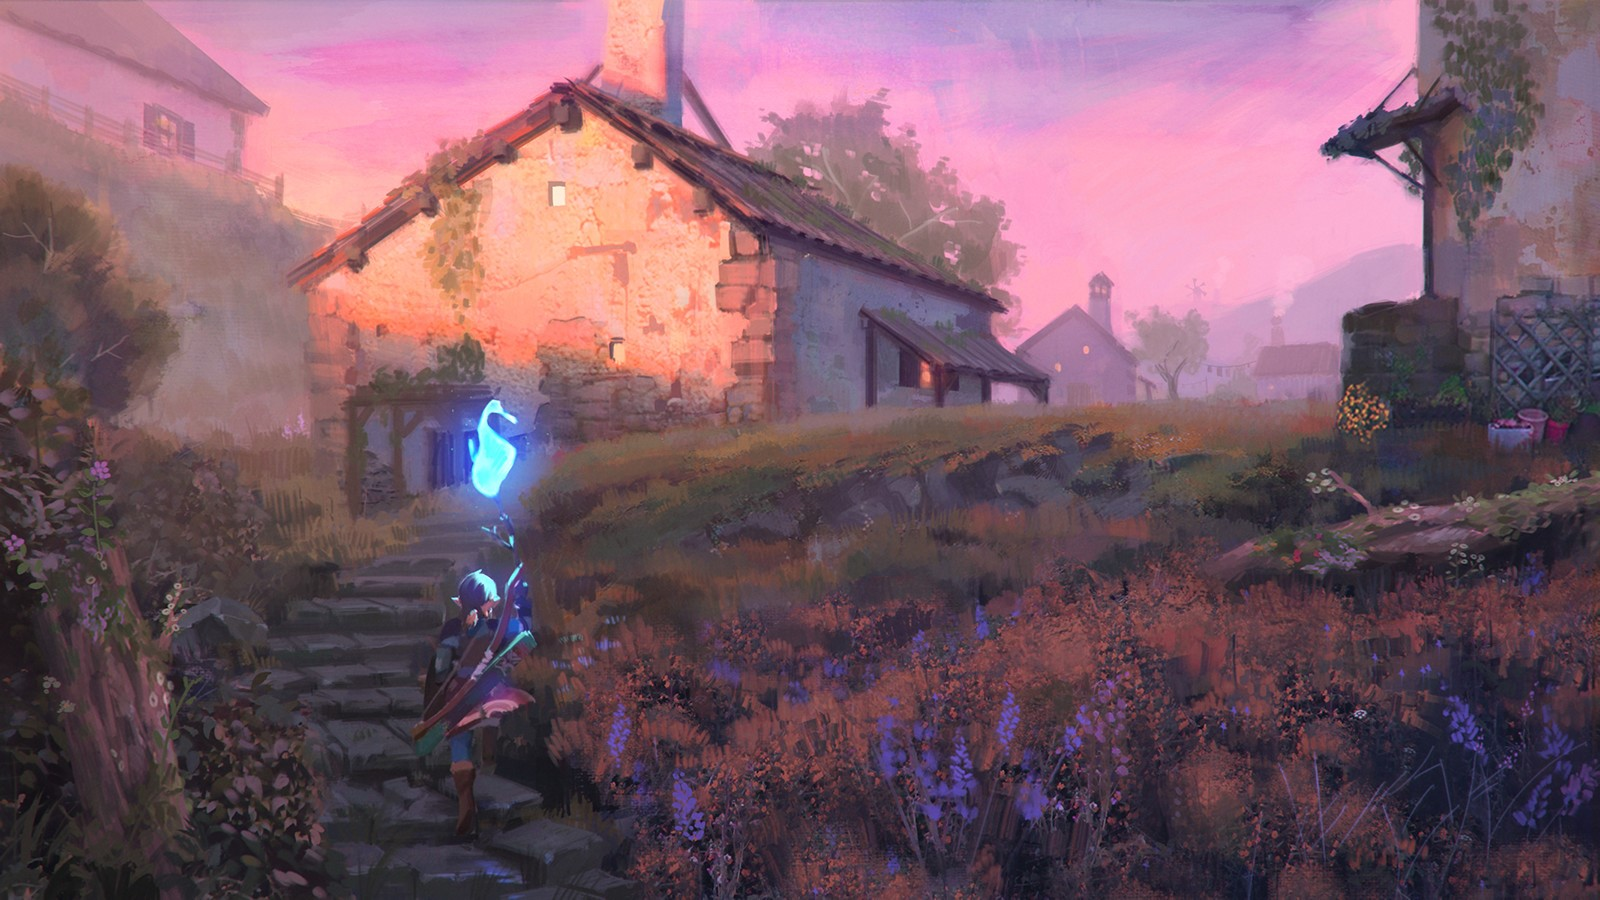
\includegraphics[scale=0.35]{images/Concepts/11_concept_art.jpg}
      \caption{\small 11. Imagen}
    \end{figure}
    Esta vez se trata de un fan art; Artista: "tacticianwinter".

        \subsubsection{Perspectiva}
        \begin{figure}[H]
      \centering
      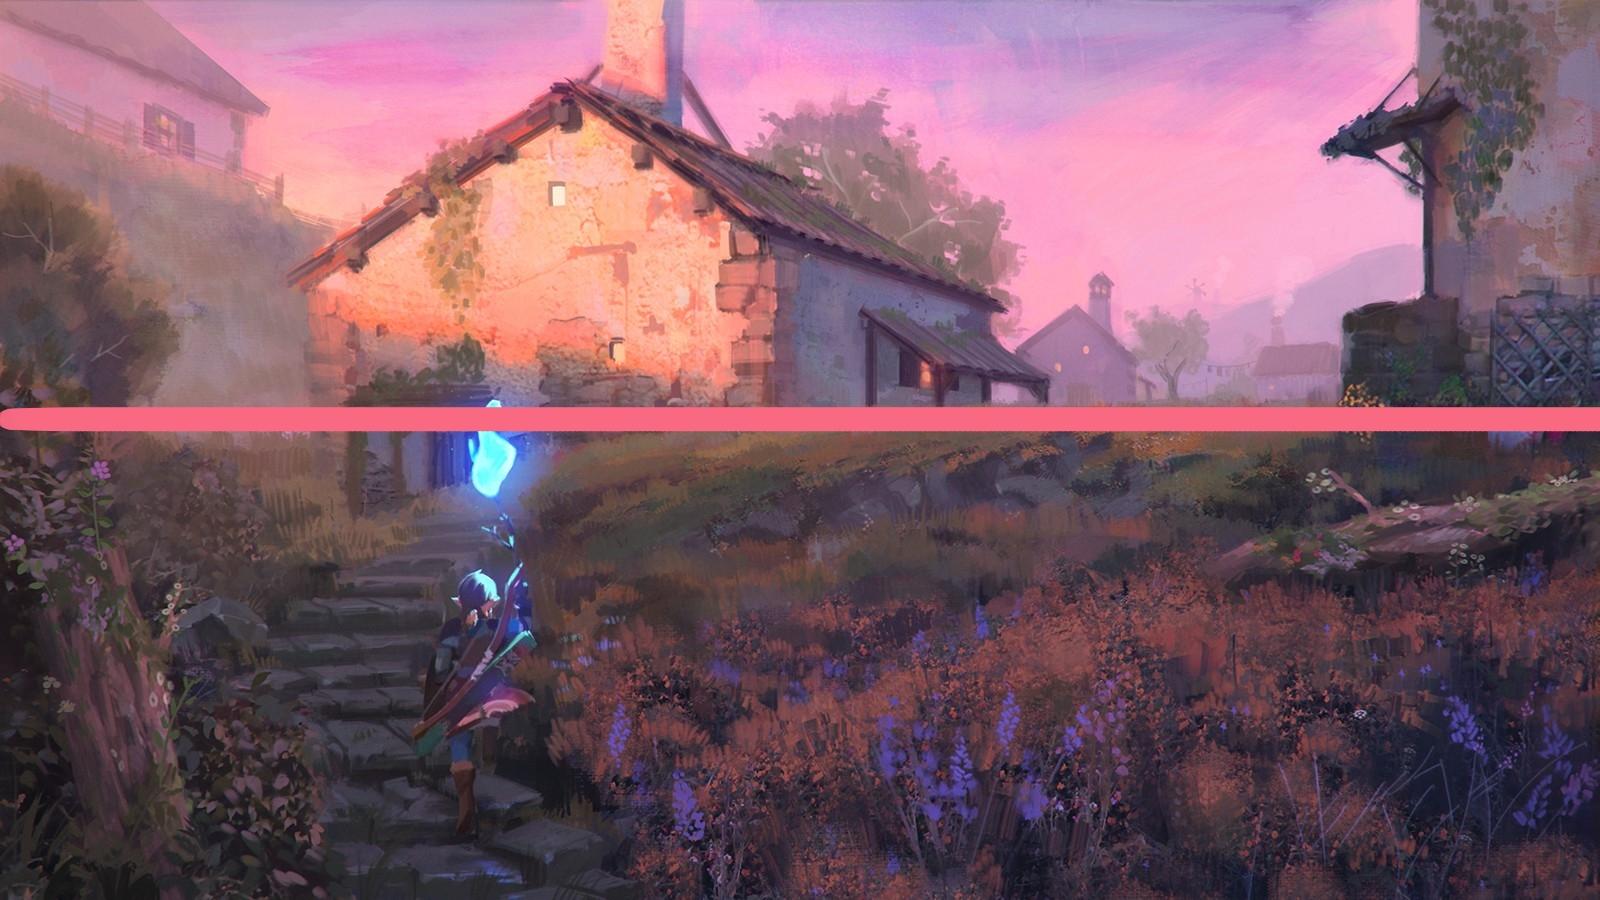
\includegraphics[scale=0.35]{images/Alonso/Sección 11/horizonte.jpg}
      \caption{\small 11. Línea de horzionte}
    \end{figure}
    Comenzaremos hablando de la línea del horizonte, la cual podemos discernir su ubicación justo en la mitad de la imagen. Ayudándonos del apoyo de las montañas en el propio horizonte podemos identificar concretamente donde se ubica este mismo. Debido a su posición podremos determinar que se trata de una vista serena.

    \begin{figure}[H]
      \centering
      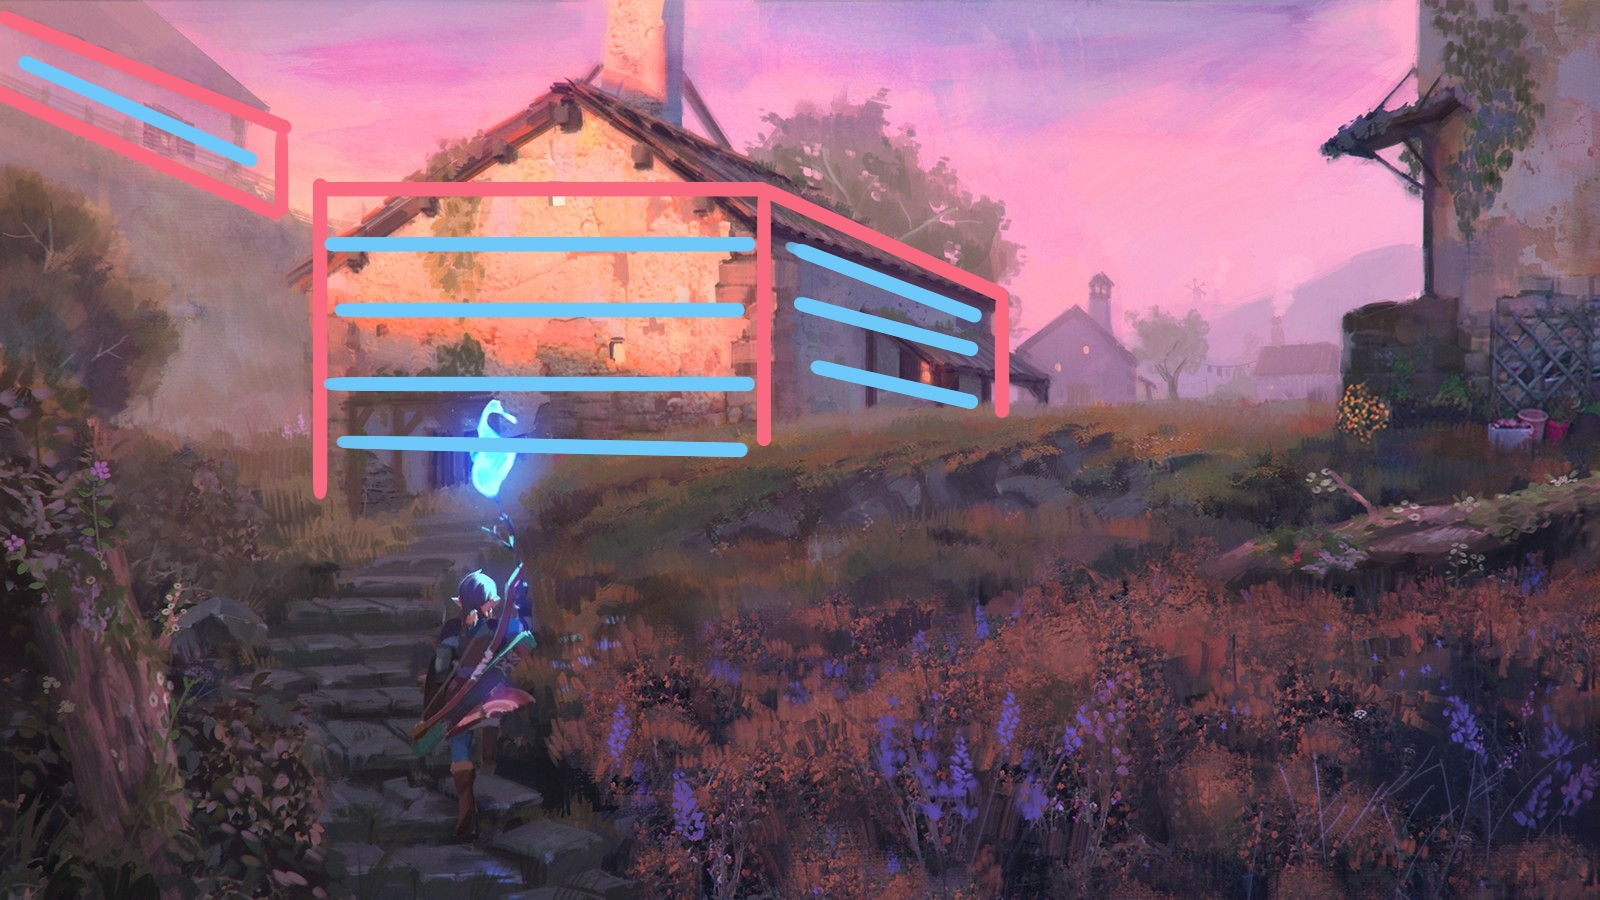
\includegraphics[scale=0.35]{images/Alonso/Sección 11/ptos de fuga.jpg}
      \caption{\small 11. Puntos de fuga}
    \end{figure}
    En esta imagen, a pesar de tener referencia de la casa no podemos determinar la posición de los puntos de fuga, pero sí que podemos determinar que como mínimo tiene 2 de ellos. Pues si nos fijamos en el cubo que representaría la casa si podemos sacar las direcciones de estos puntos de fuga, y la existencia de estos mismos.

        \subsubsection{Composición}
        \begin{figure}[H]
      \centering
      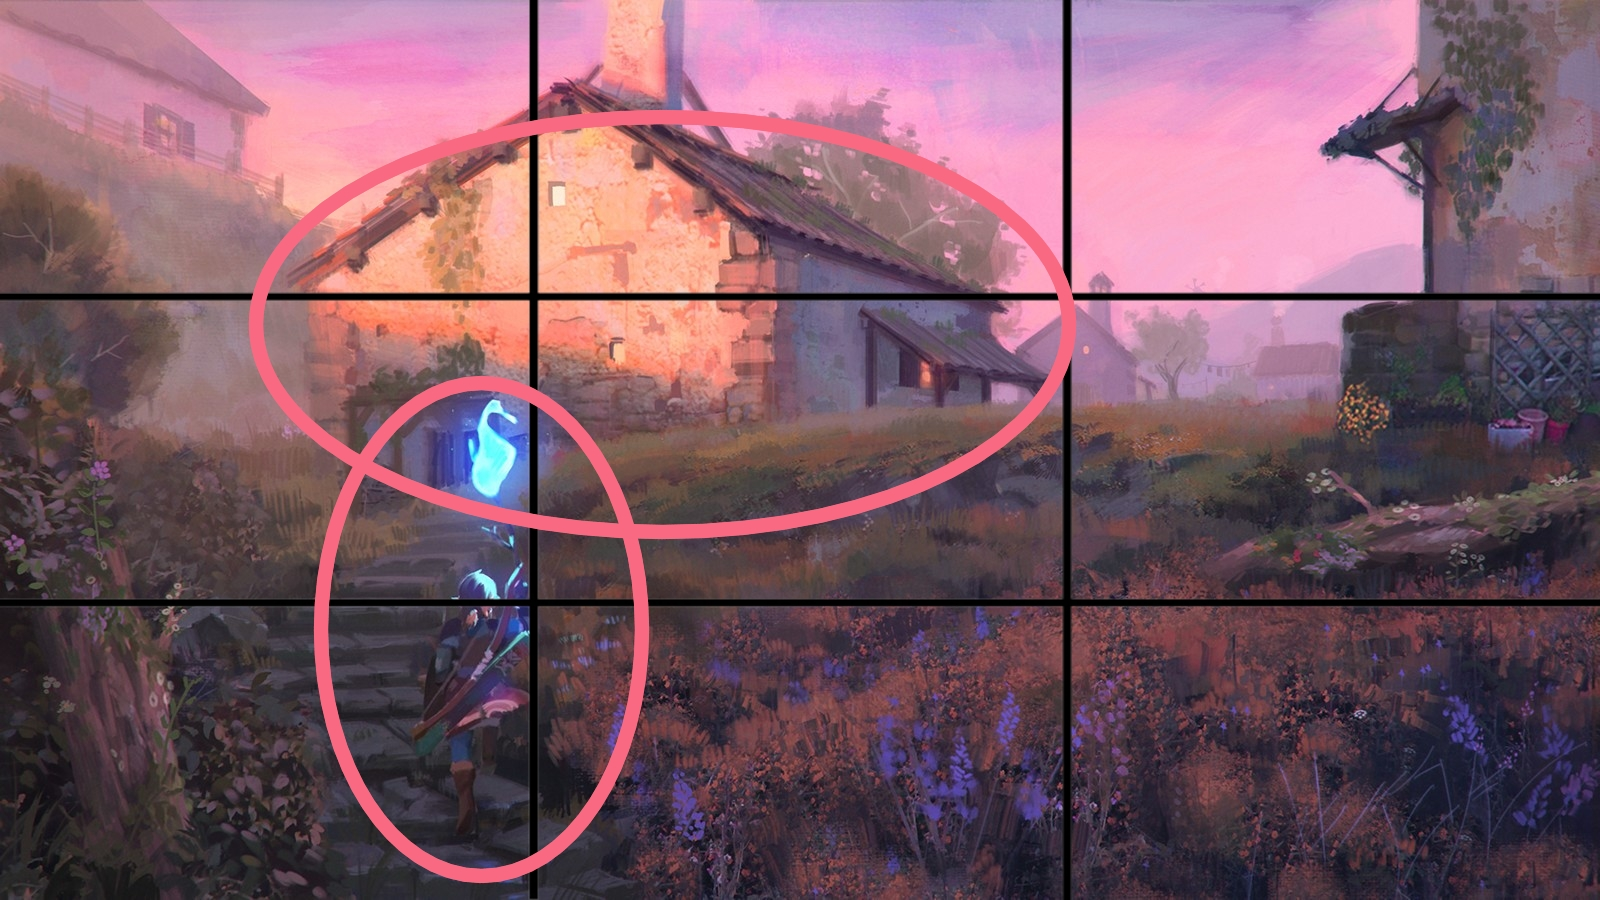
\includegraphics[scale=0.35]{images/Alonso/Sección 11/tercios.jpg}
      \caption{\small 11. 2/3}
    \end{figure}
     En la regla de los 2/3  podemos ver como las esquinas señalaron a los elementos más notorios de la imagen, siendo estos los puntos de interés más importantes en toda la imagen.

    \begin{figure}[H]
      \centering
      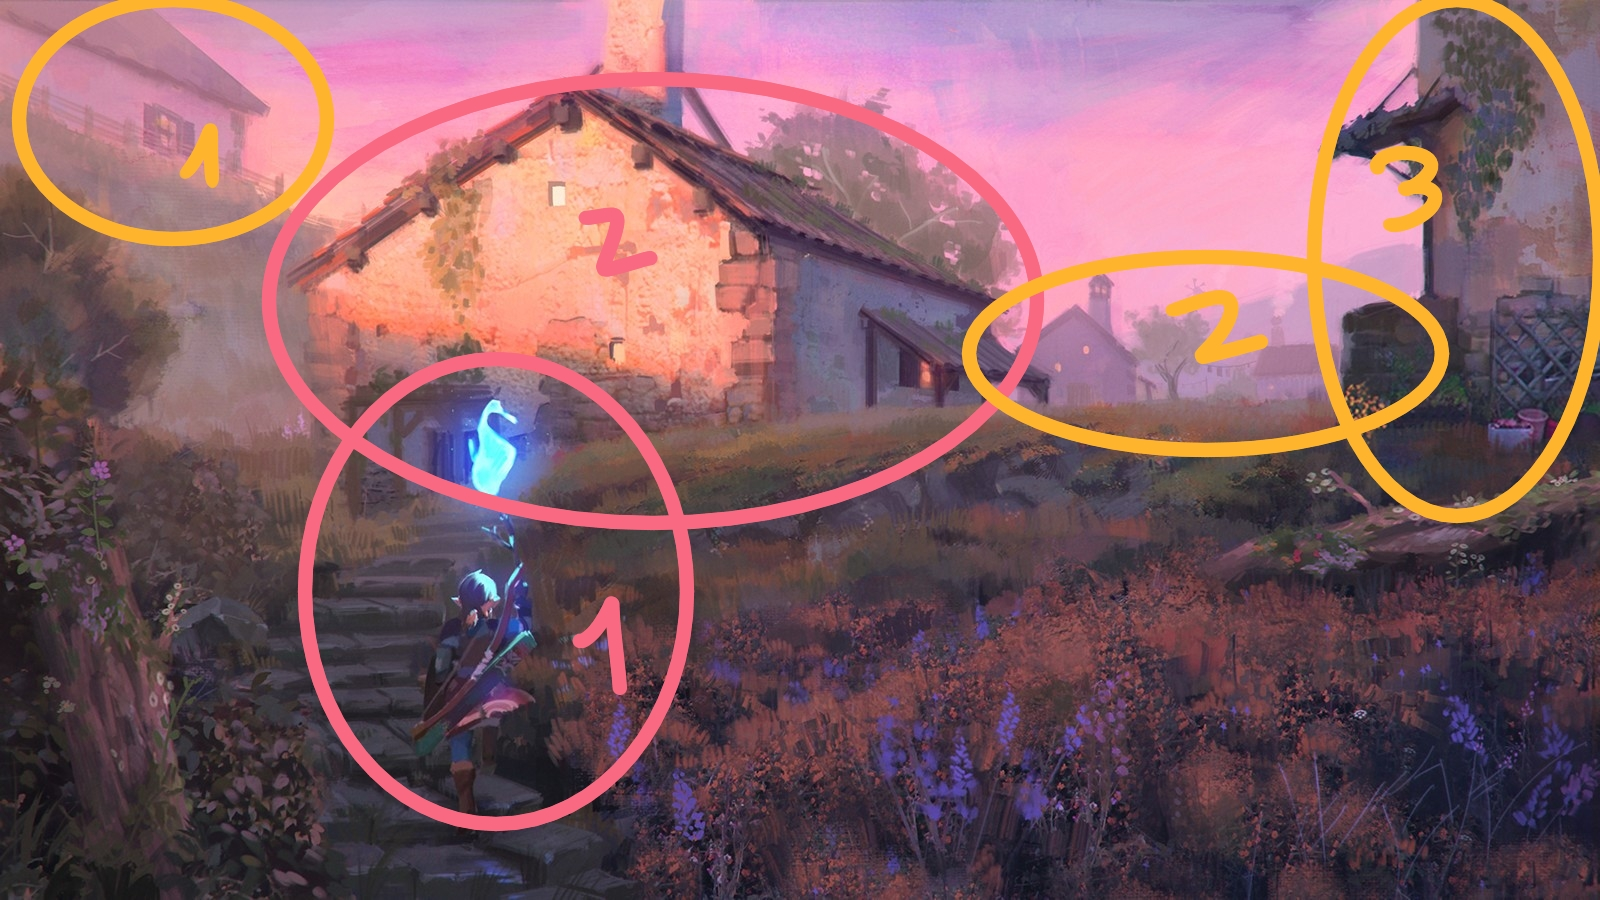
\includegraphics[scale=0.35]{images/Alonso/Sección 11/ptos de interes.jpg}
      \caption{\small 11. puntos de interes}
    \end{figure}
    Además de estar situados ahí en las esquinas, la luminosidad juega un gran papel a la hora de seleccionar estos putos como los más importantes de la imagen. Pues el punto principal se trataría de Link, por ser un gran contraste de tono, tanto como su ropa como la antorcha azul resaltan con el fondo. Y la casa es la única iluminada por el rayo de sol.
    También podremos denotar más puntos de interés, pero estos siendo secundarios, como podría ser el porche de la derecha de la imagen como las pocas casas que hay en el fondo al ser elementos grandes en la imagen.

    \begin{figure}[H]
      \centering
      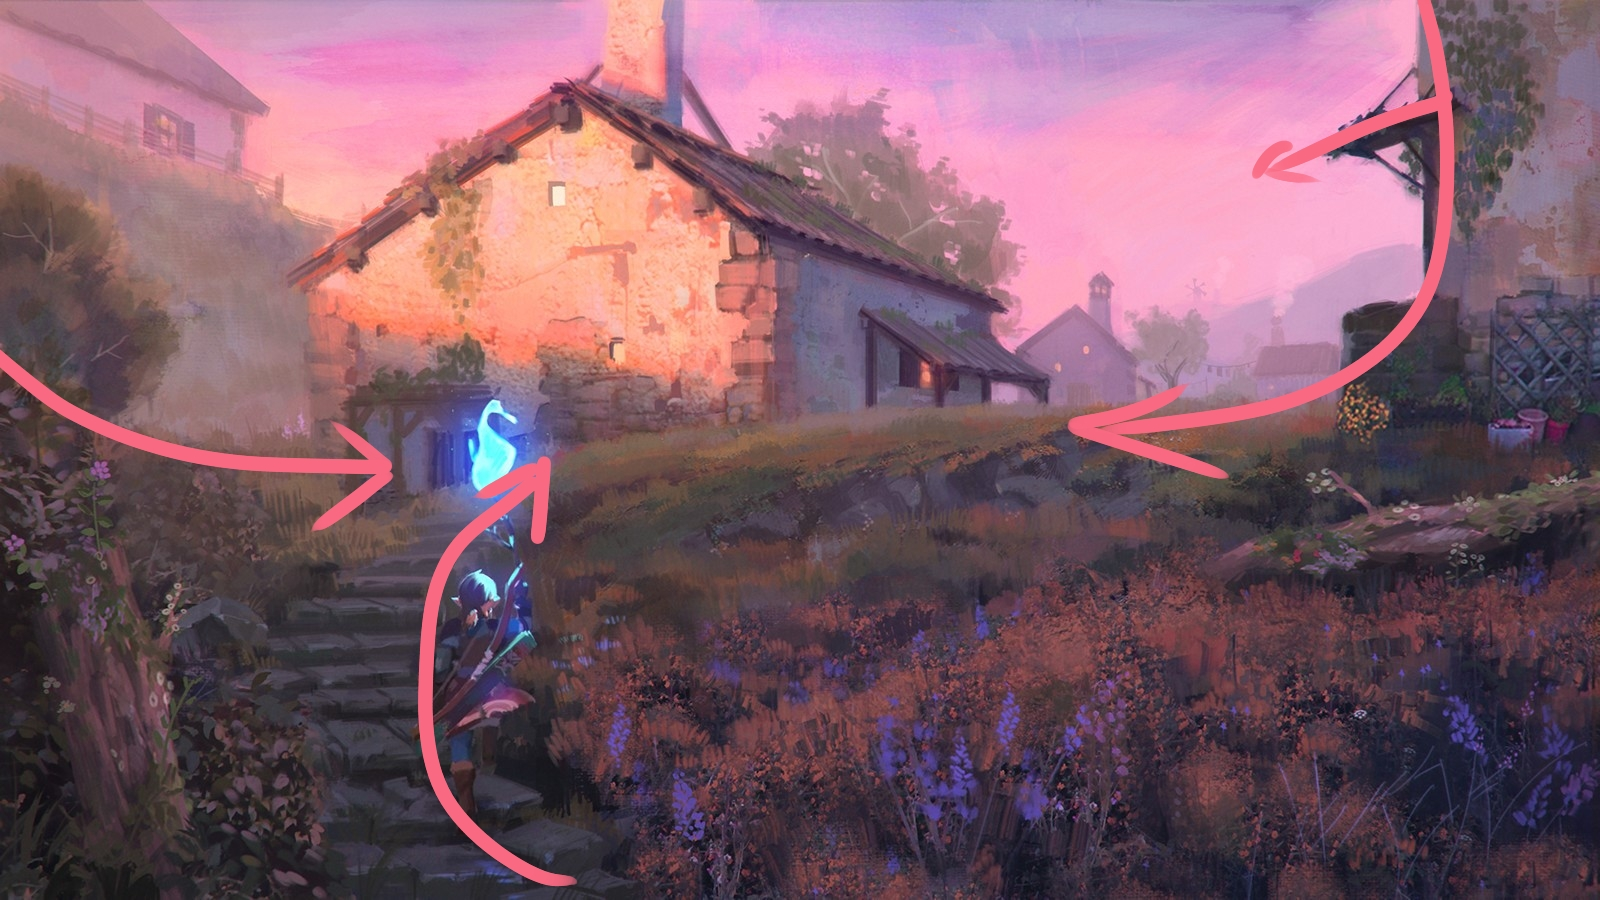
\includegraphics[scale=0.35]{images/Alonso/Sección 11/recorridos visuales.jpg}
      \caption{\small 11. recorrido visual}
    \end{figure}
    El recorrido visual es bastante claro gracias al camino de piedra por el que anda Link, haciendo una pequeña curva hacia la casa, tanto la mirada como el recorrido de su pose señalan también a la luz que ilumina la propia casa. Es más, la propia inclinación del terreno nos podría dar pistas de en que quiere que nos enfoquemos la imagen, que es en ese gran punto de luz situado en la casa.

\begin{figure}[H]
      \centering
      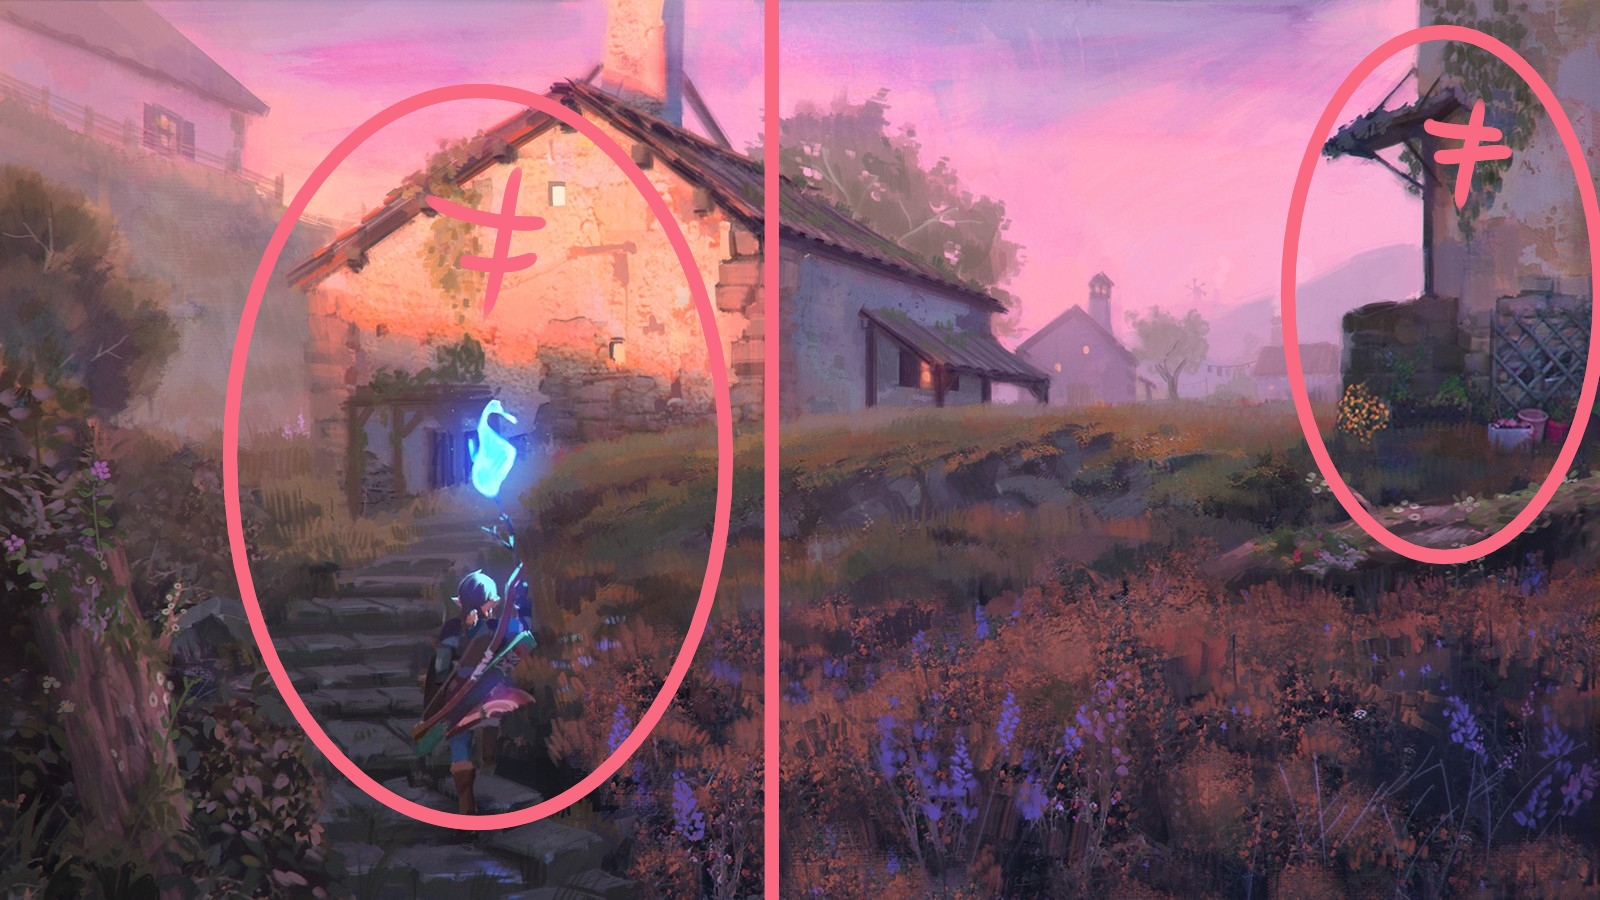
\includegraphics[scale=0.35]{images/Alonso/Sección 11/balanza.jpg}
      \caption{\small 11. ley Balanza}
    \end{figure}
    La ley de la balanza y los pesos es rápido determinar que no se cumple, pues el lado izquierdo asume mucho más contenido e información a la imagen que el oscuro y recóndito sitio que nos brinda el lado derecho. Aprovechando la propia línea podemos ver que no se cumple la simetría en ningún punto.


        \subsubsection{Clarooscuro}
        \begin{figure}[H]
      \centering
      \includegraphics[scale=0.35]{images/Alonso/Sección 11/blanco y negro.jpg}
      \caption{\small 11. Profundidad}
    \end{figure}
    Si desaturamos toda la imagen nos podremos dar cuenta de que apenas hay un gran contraste y diferenciación entre un primer y segundo plano, pero sí puede discernirse ligeramente debido a la luz de la parte superior de la imagen que nos hace un efecto de profundidad notorio en la composición.

    \begin{figure}[H]
      \centering
      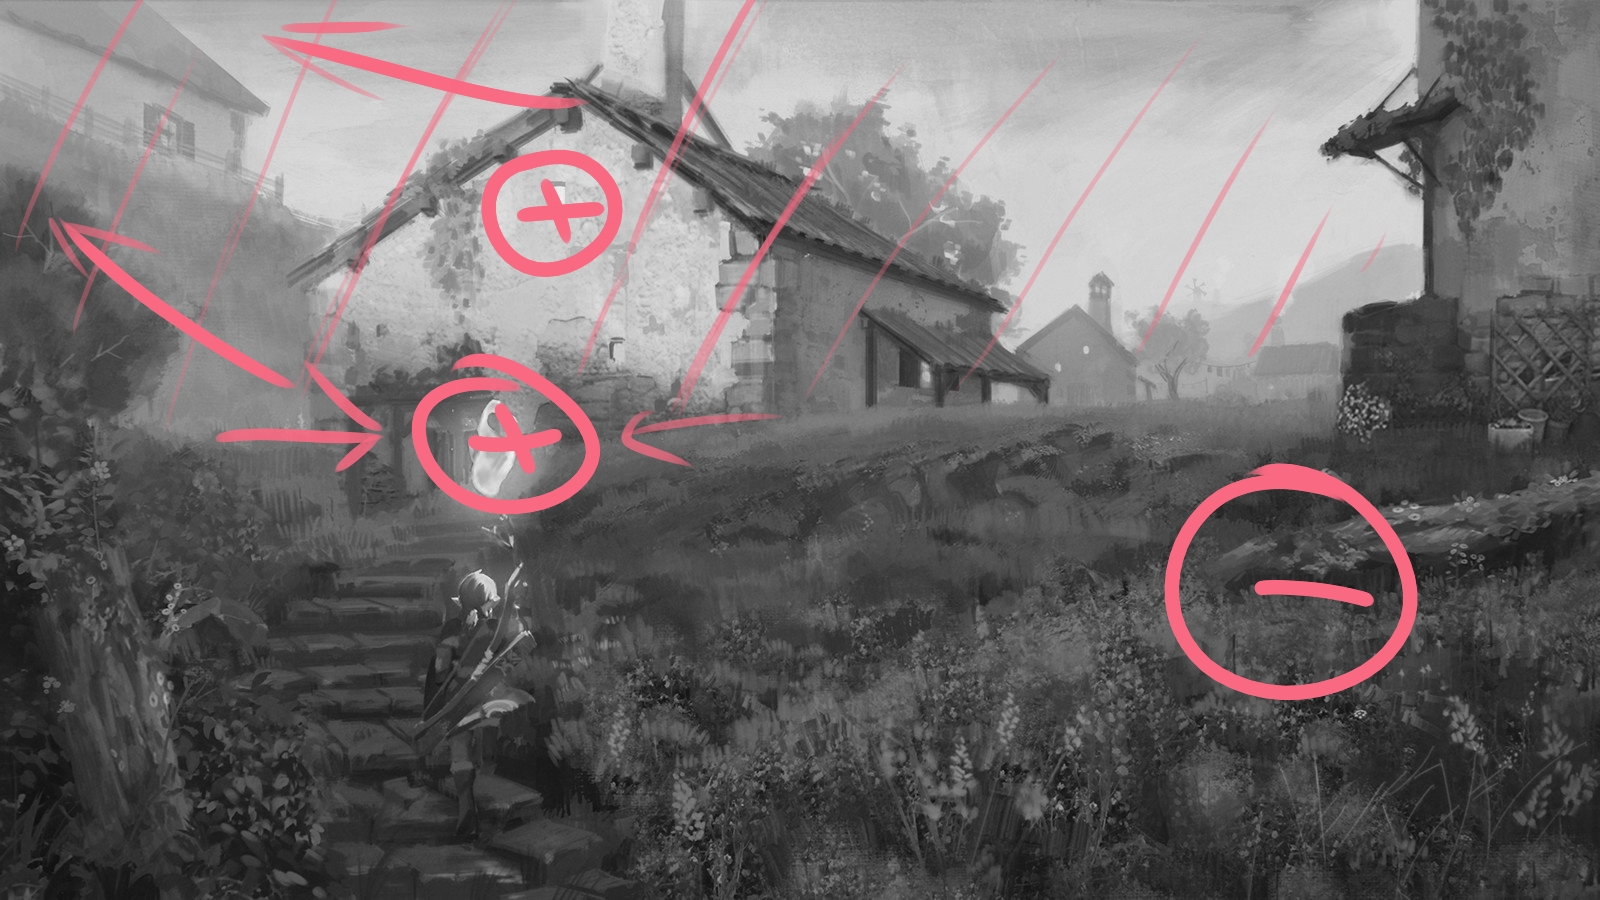
\includegraphics[scale=0.35]{images/Alonso/Sección 11/iluminacion.jpg}
      \caption{\small 11. Fuente de luz}
    \end{figure}

    Además podemos ver desde donde procede la luz y es que tenemos dos fuentes de luz en la imagen, primero podemos ver el sol que ilumina la casa que es la parte que más iluminada esta de la casa. El segundo foco de luz lo podemos ver en la mano de link, la antorcha que sujeta. A pesar de ello la antorcha no ilumina mucho más allá del ropaje de link.

\begin{figure}[H]
      \centering
      \includegraphics[scale=0.35]{images/Alonso/Sección 11/pixel.jpg}
      \caption{\small 11. pixelado}
    \end{figure}

    Si pixelamos la imagen debido a la poca luz que proporciona el atardecer de la imagen podemos ver que se trata de una clave media

        \subsubsection{Color}
\begin{figure}[H]
      \centering
      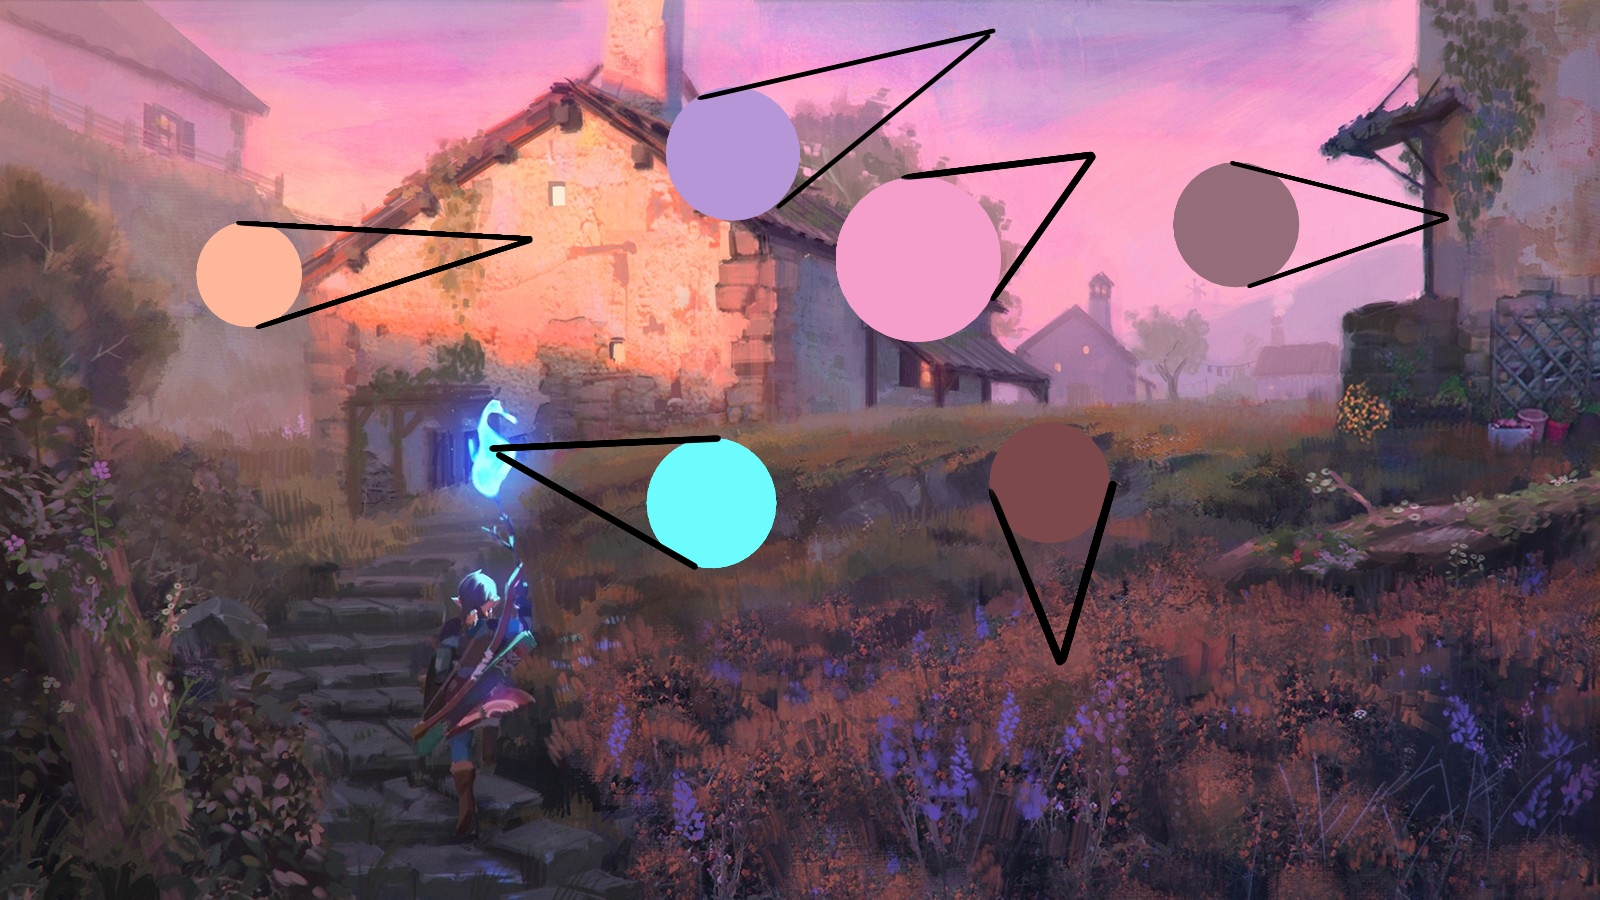
\includegraphics[scale=0.35]{images/Alonso/Sección 11/gamacolorifica.jpg}
      \caption{\small 11. Gama de colores}
    \end{figure}

        Si hacemos un análisis del tono global de la imagen no existe una relación sólida entre los diferentes tonos repartidos por toda la composición. Sin embargo podemos observar que las zonas de estos tonos, están rodeadas de unos colores análogos.

        \begin{figure}[H]
      \centering
      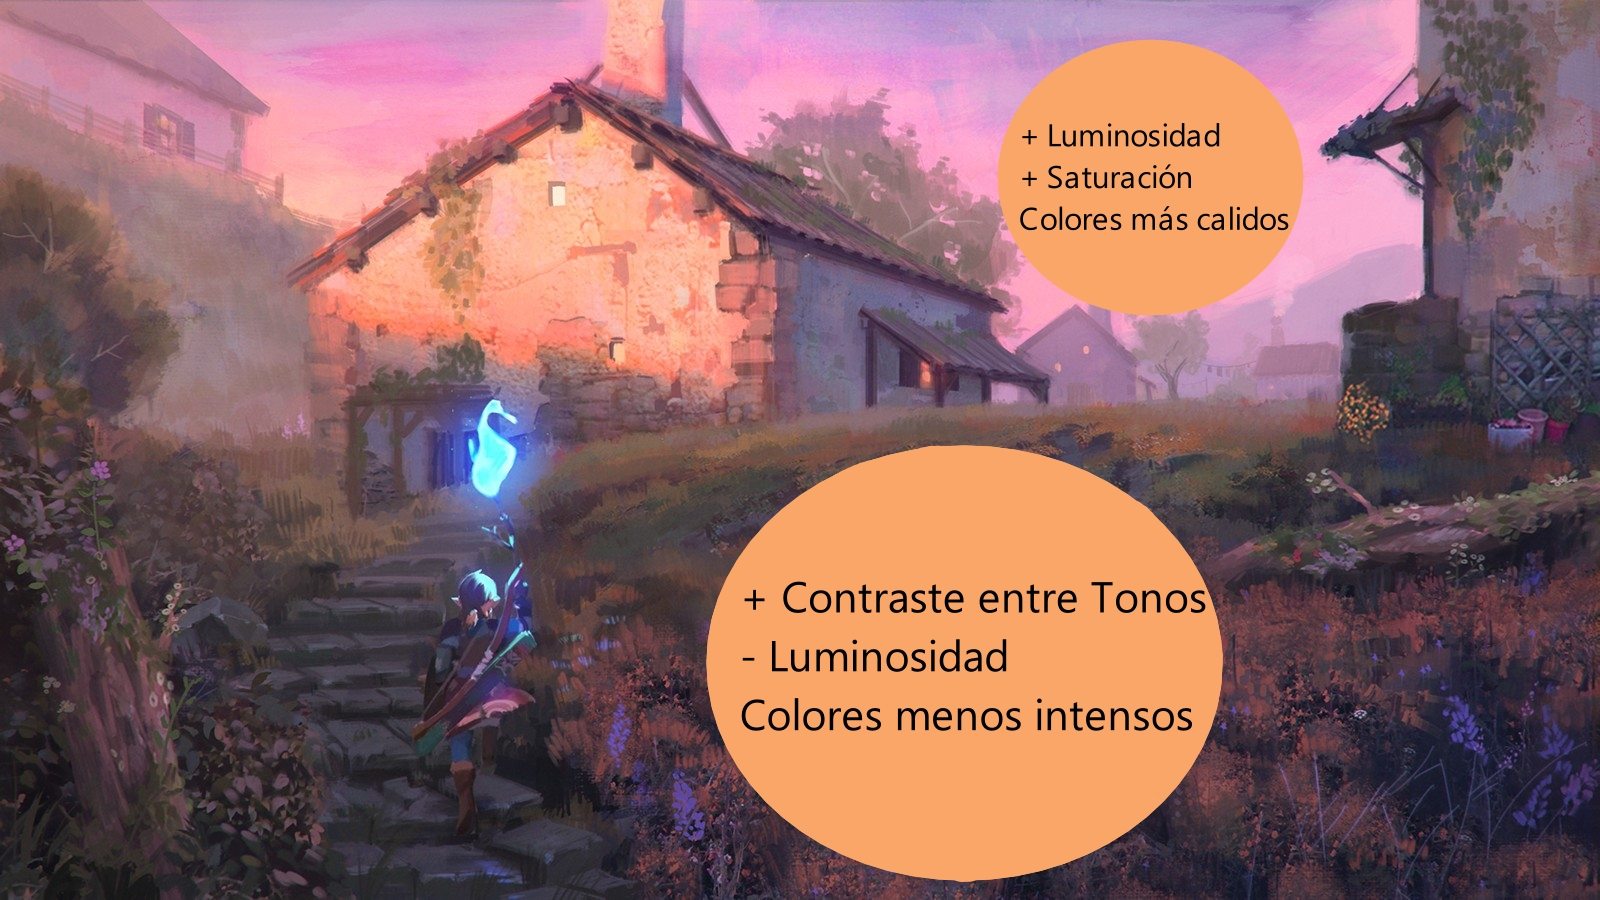
\includegraphics[scale=0.35]{images/Alonso/Sección 11/planos.jpg}
      \caption{\small 11. Gama de colores}
    \end{figure}
    En primer plano también nos brinda una serie de tonos cálidos pero con menos saturacion y pequeños atisbos de una gama de color más fria debido a la sombra y la poca iluminosidad que existe en esta zona. en segundo plano  podemos ver que el cielo está compuesto por una serie de colores cálidos análogos.

    \begin{figure}[H]
      \centering
      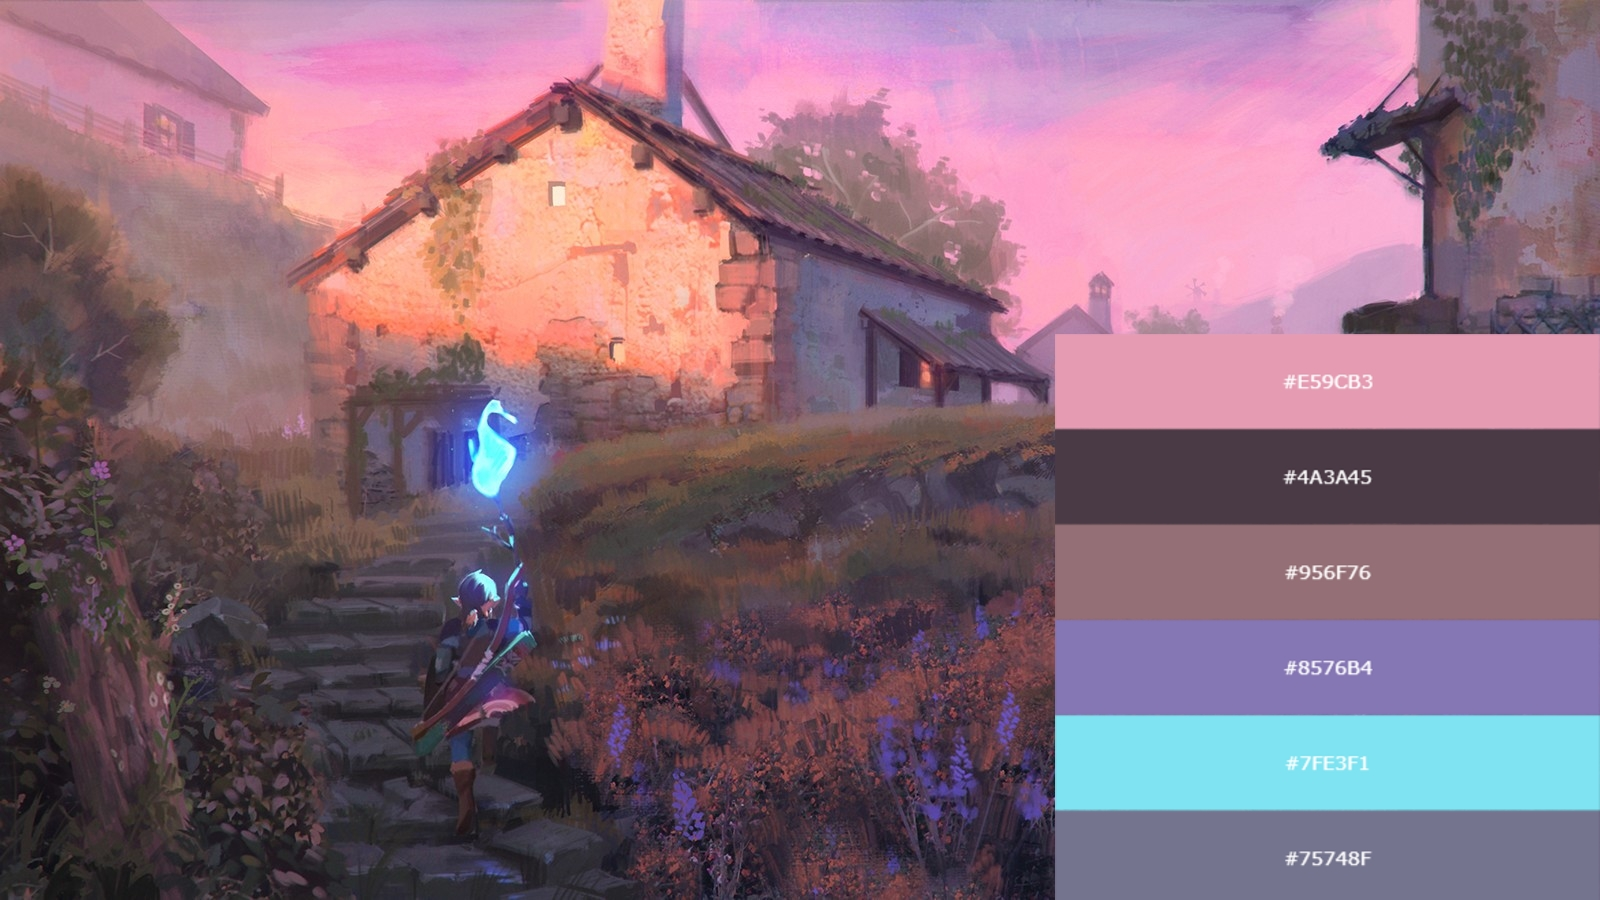
\includegraphics[scale=0.35]{images/Alonso/Sección 11/tonalidad paletil.jpg}
      \caption{\small 11. paleta de colores}
    \end{figure}

    De todas formas este es la gama de colores que se ha empleado a la hora de hacer la imagen.

\begin{figure}[H]
      \centering
      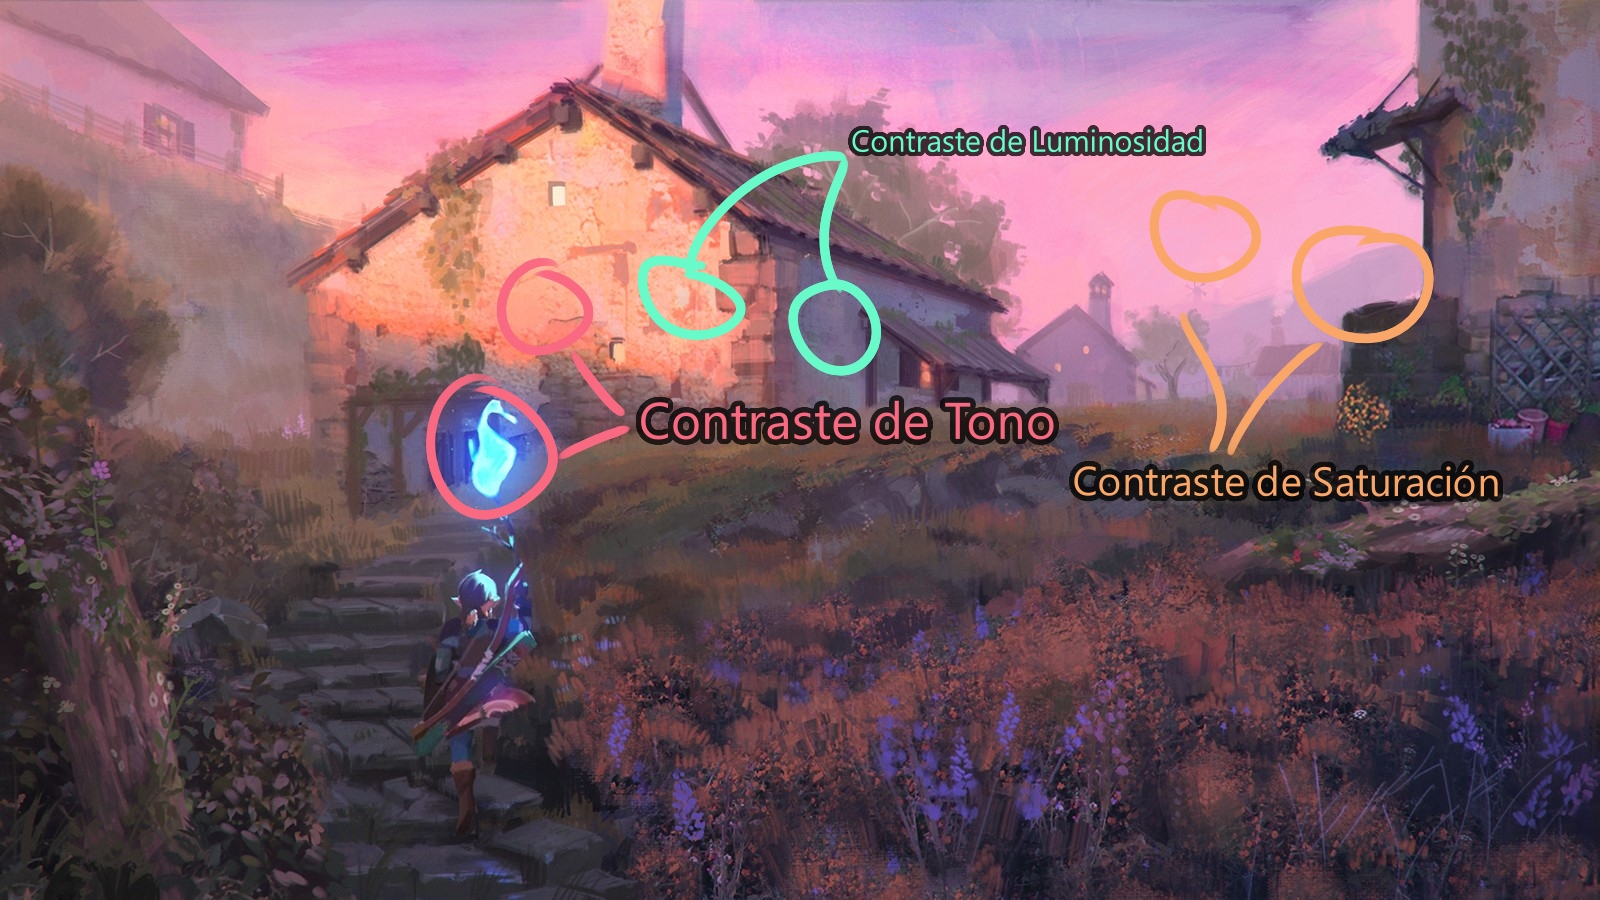
\includegraphics[scale=0.35]{images/Alonso/Sección 11/constrastes.jpg}
      \caption{\small 11. Contrastes}
    \end{figure}
    Para terminar hay bastantes zonas de contraste en la imagen, para empezar un claro ejemplo de contraste de tono sería irnos hacia link y ver que todos los colores del ambiente que lo rodean son totalmente diferentes al azul eléctrico que nos brinda su antorcha y ropajes. El contraste de luminosidad se expone en la casa, pues la parte del sol deja ver un luminoso color anaranjado y en la parte oscura un apagado color naranja. Para terminar su contraste de saturación es menos evidente. Pero podemos ver el fondo del cielo, una zona menos saturada en la que se encuentran las montañas y el cielo iluminado con un color rosado.
        \newpage

%-----------------------------------------------------------------
%-----------------------------------------------------------------

    \subsection{12. Carlos}
        \subsubsection{Perspectiva}

        \subsubsection{Composición}

        \subsubsection{Clarooscuro}

        \subsubsection{Color}
        \newpage

%-----------------------------------------------------------------
%-----------------------------------------------------------------

    \subsection{13. Joan}
        \subsubsection{Perspectiva}

        \subsubsection{Composición}

        \subsubsection{Clarooscuro}

        \subsubsection{Color}
        \newpage

%-----------------------------------------------------------------
%-----------------------------------------------------------------

    \subsection{14. Selena (Segunda imagen)}
        \subsubsection{Perspectiva}

        \subsubsection{Composición}

        \subsubsection{Clarooscuro}

        \subsubsection{Color}
        \newpage

%-----------------------------------------------------------------
%-----------------------------------------------------------------

    \subsection{15. Carlos (Segunda Imagen)}
        \subsubsection{Perspectiva}

        \subsubsection{Composición}

        \subsubsection{Clarooscuro}

        \subsubsection{Color}
        \newpage

%-----------------------------------------------------------------
%-----------------------------------------------------------------

    \subsection{16. Jesus}
        \subsubsection{Perspectiva}

        \subsubsection{Composición}

        \subsubsection{Clarooscuro}

        \subsubsection{Color}
        \newpage

%-----------------------------------------------------------------
%-----------------------------------------------------------------

    \subsection{17. Saul (Segunda Imagen)}
    \begin{figure}[H]
      \centering
      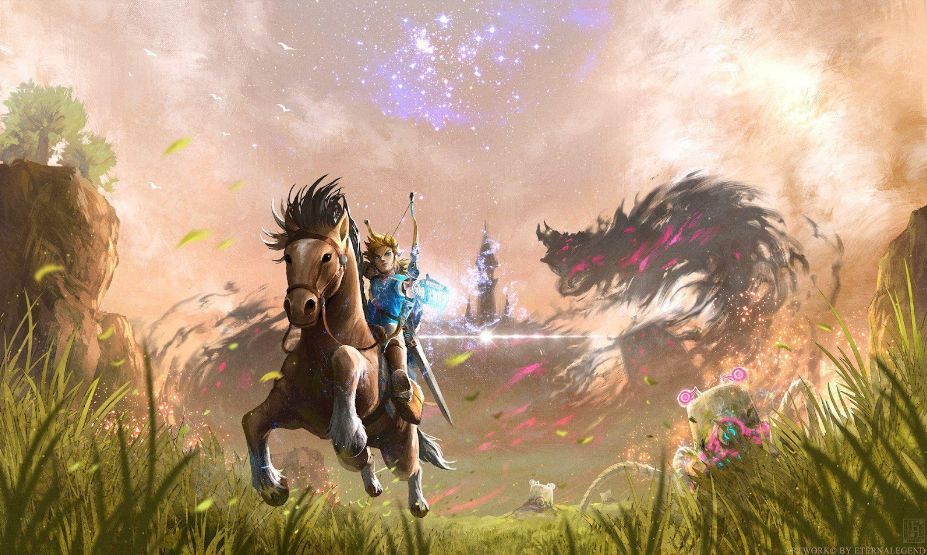
\includegraphics[scale=0.7]{images/Saúl/Sección 17/EA_img17_0Main.png}
      \caption{\small 4.3.3. Imagen}
    \end{figure}
    Se trata de una imagen oficial del juego, y se compone por el personaje principal montado a su caballo Epona, disparando una flecha y al fondo tenemos el castillo de Hyrule con Gandondorf que es el villano del videojuego.

    
        \subsubsection{Análisis de la perspectiva}


    \begin{figure}[H]
      \centering
      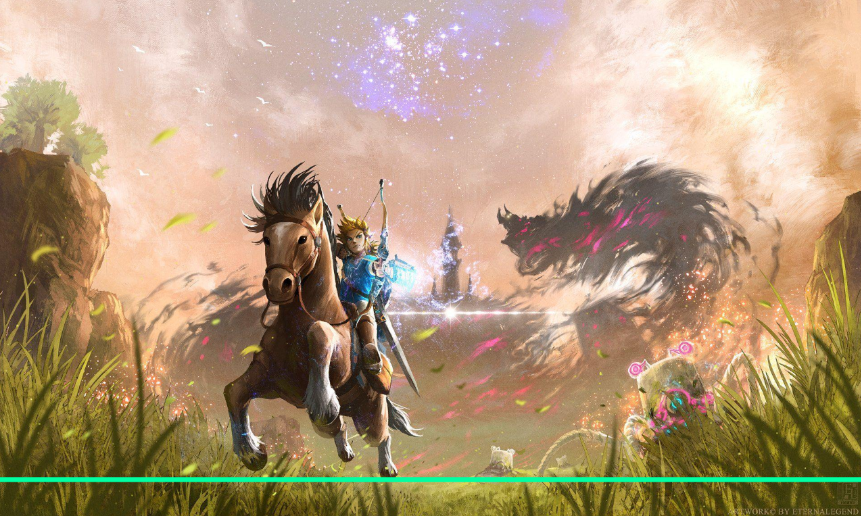
\includegraphics[scale=0.7]{images/Saúl/Sección 17/EA_img17_1Perspectiva_1LineaTierra-TipoVista.png}
      \caption{\small 4.3.1.1 Línea del horizonte y tipo de vista}
    \end{figure}



    \begin{figure}[H]
      \centering
      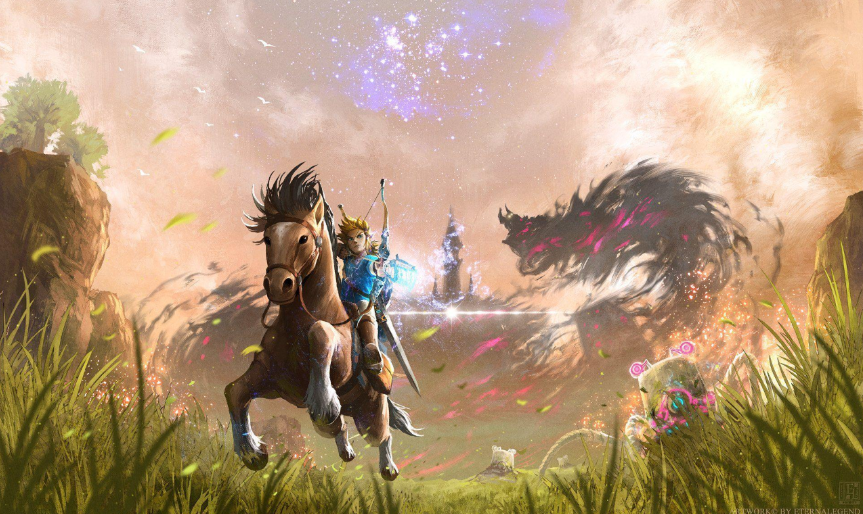
\includegraphics[scale=0.7]{images/Saúl/Sección 17/EA_img17_1Perspectiva_2PuntosFuga.png}
      \caption{\small 4.3.1.2 Puntos de fuga}
    \end{figure}




        \subsubsection{Análisis de la composición}

        
    \begin{figure}[H]
      \centering
      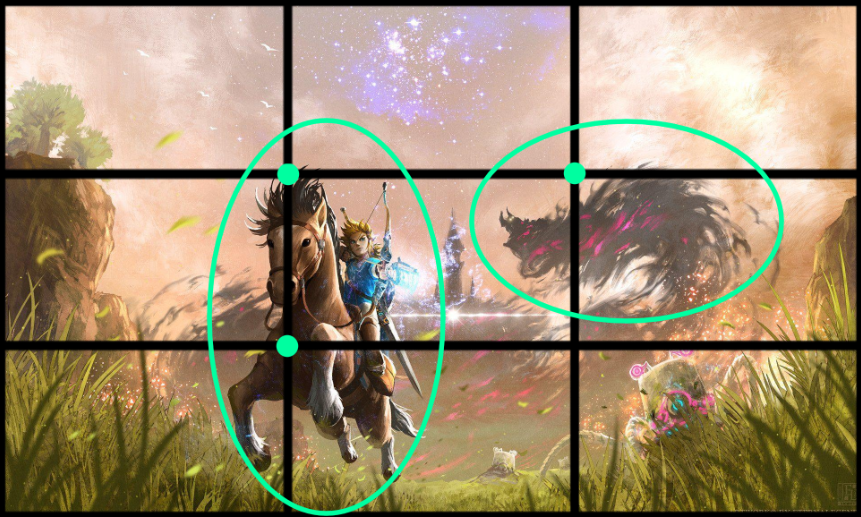
\includegraphics[scale=0.7]{images/Saúl/Sección 17/EA_img17_2Composicion_1Regla2-3.png}
      \caption{\small 4.3.2.1 Regla de los 2/3}
    \end{figure}



    \begin{figure}[H]
      \centering
      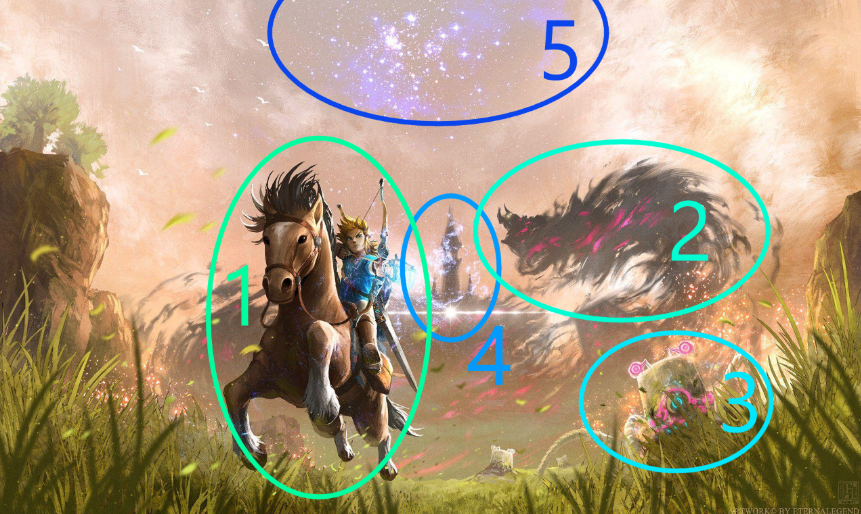
\includegraphics[scale=0.7]{images/Saúl/Sección 17/EA_img17_2Composicion_2PuntosInteres.png}
      \caption{\small 4.3.2.2 Centro de interés, principal y secundarios}
    \end{figure}



    \begin{figure}[H]
      \centering
      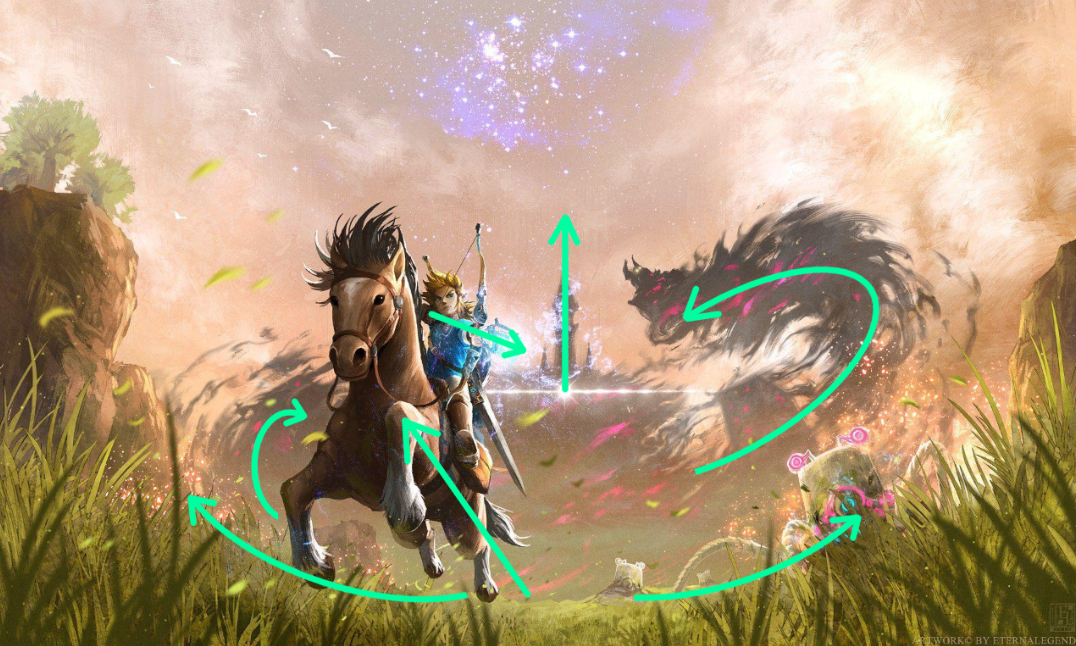
\includegraphics[scale=0.7]{images/Saúl/Sección 17/EA_img17_2Composicion_3RutaVisual.png}
      \caption{\small 4.3.2.3 Ruta visual}
    \end{figure}



    \begin{figure}[H]
      \centering
      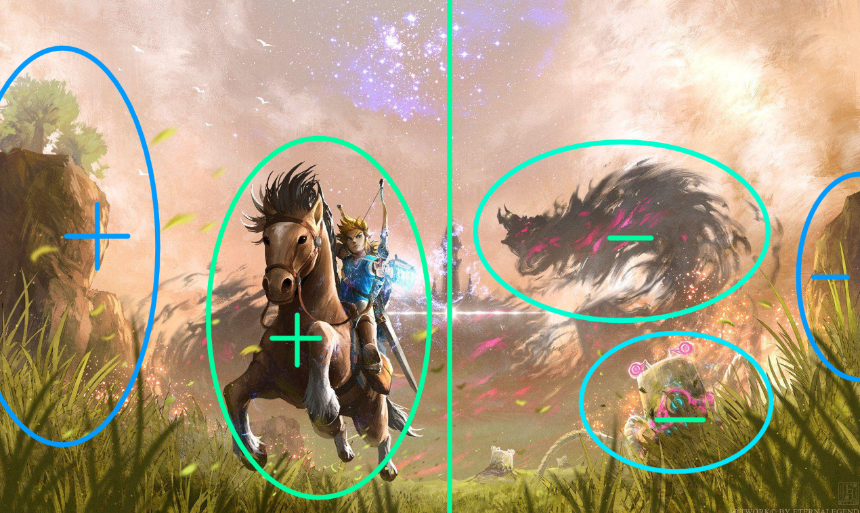
\includegraphics[scale=0.7]{images/Saúl/Sección 17/EA_img17_2Composicion_4LeyBalanza-Simetria.png}
      \caption{\small 4.3.2.4 Ley de la balanza, equilibrio de pesos y simetría vs asimetría}
    \end{figure}





        \subsubsection{Claroscuro}

        
    \begin{figure}[H]
      \centering
      \includegraphics[scale=0.7]{images/Saúl/Sección 17/EA_img17_3Claroscuro_1Profundidad.png}
      \caption{\small 4.3.3.1 Uso del claroscuro para representar la profundidad}
    \end{figure}



    \begin{figure}[H]
      \centering
      \includegraphics[scale=0.7]{images/Saúl/Sección 17/EA_img17_3Claroscuro_2Luminosidad.png}
      \caption{\small 4.3.3.2 Zonas más luminosas y menos, y ubicación de la fuente de iluminación}
    \end{figure}


    \begin{figure}[H]
      \centering
      \includegraphics[scale=0.7]{images/Saúl/Sección 17/EA_img17_3Claroscuro_3Clave.png}
      \caption{\small 4.3.3.3 Clave de la imagen}
    \end{figure}



        \subsubsection{Color}


    \begin{figure}[H]
      \centering
      \includegraphics[scale=0.7]{images/Saúl/Sección 17/EA_img17_4Color_1TonalidadGenral.png}
      \caption{\small 4.3.4.1 Tonalidad de color global}
    \end{figure}



    \begin{figure}[H]
      \centering
      \includegraphics[scale=0.7]{images/Saúl/Sección 17/EA_img17_4Color_2GamaColores.png}
      \caption{\small 4.3.4.2 Gama de color empleada}
    \end{figure}



    \begin{figure}[H]
      \centering
      \includegraphics[scale=0.7]{images/Saúl/Sección 17/EA_img17_4Color_3Contrastes.png}
      \caption{\small 4.3.4.3 Tipos de contraste}
    \end{figure}



    \begin{figure}[H]
      \centering
      \includegraphics[scale=0.7]{images/Saúl/Sección 17/EA_img17_4Color_4AnalisisPlanosPrimeroFondo.png}
      \caption{\small 4.3.4.4 Análisis de los colores empleados en primer y último plano}
    \end{figure}


        \newpage

%-----------------------------------------------------------------
%-----------------------------------------------------------------

    \subsection{18. Joan (Segunda Imagen)}
        \subsubsection{Perspectiva}

        \subsubsection{Composición}

        \subsubsection{Clarooscuro}

        \subsubsection{Color}
        
\end{document}